%Version 3.1 December 2024
% See section 11 of the User Manual for version history
%
%%%%%%%%%%%%%%%%%%%%%%%%%%%%%%%%%%%%%%%%%%%%%%%%%%%%%%%%%%%%%%%%%%%%%%
%%                                                                 %%
%% Please do not use \input{...} to include other tex files.       %%
%% Submit your LaTeX manuscript as one .tex document.              %%
%%                                                                 %%
%% All additional figures and files should be attached             %%
%% separately and not embedded in the \TeX\ document itself.       %%
%%                                                                 %%
%%%%%%%%%%%%%%%%%%%%%%%%%%%%%%%%%%%%%%%%%%%%%%%%%%%%%%%%%%%%%%%%%%%%%

%%\documentclass[referee,sn-basic]{sn-jnl}% referee option is meant for double line spacing

%%=======================================================%%
%% to print line numbers in the margin use lineno option %%
%%=======================================================%%

%%\documentclass[lineno,pdflatex,sn-basic]{sn-jnl}% Basic Springer Nature Reference Style/Chemistry Reference Style

%%=========================================================================================%%
%% the documentclass is set to pdflatex as default. You can delete it if not appropriate.  %%
%%=========================================================================================%%

%%\documentclass[sn-basic]{sn-jnl}% Basic Springer Nature Reference Style/Chemistry Reference Style

%%Note: the following reference styles support Namedate and Numbered referencing. By default the style follows the most common style. To switch between the options you can add or remove “Numbered” in the optional parenthesis. 
%%The option is available for: sn-basic.bst, sn-chicago.bst%  
 
%%\documentclass[pdflatex,sn-nature]{sn-jnl}% Style for submissions to Nature Portfolio journals
%%\documentclass[pdflatex,sn-basic]{sn-jnl}% Basic Springer Nature Reference Style/Chemistry Reference Style
\PassOptionsToPackage{table}{xcolor}
\documentclass[pdflatex,sn-mathphys-num]{sn-jnl}% Math and Physical Sciences Numbered Reference Style
%%\documentclass[pdflatex,sn-mathphys-ay]{sn-jnl}% Math and Physical Sciences Author Year Reference Style
%%\documentclass[pdflatex,sn-aps]{sn-jnl}% American Physical Society (APS) Reference Style
%%\documentclass[pdflatex,sn-vancouver-num]{sn-jnl}% Vancouver Numbered Reference Style
%%\documentclass[pdflatex,sn-vancouver-ay]{sn-jnl}% Vancouver Author Year Reference Style
%%\documentclass[pdflatex,sn-apa]{sn-jnl}% APA Reference Style
%%\documentclass[pdflatex,sn-chicago]{sn-jnl}% Chicago-based Humanities Reference Style

%%%% Standard Packages
%%<additional latex packages if required can be included here>

\usepackage{graphicx}%
\usepackage{multirow}%
\usepackage{amsmath,amssymb,amsfonts}%
\usepackage{amsthm}%
\usepackage{mathrsfs}%
\usepackage[title]{appendix}%
\usepackage{xcolor}%
\usepackage{textcomp}%
\usepackage{manyfoot}%
\usepackage{booktabs}%
\usepackage{algorithm}%
\usepackage{algorithmicx}%
\usepackage{algpseudocode}%
\usepackage{listings}%
\usepackage{array}%
\usepackage{tikz}%
\usetikzlibrary{positioning,arrows.meta,fit,calc}%
\graphicspath{{figures/}}%
%%%%

%%%%%=============================================================================%%%%
%%%%  Remarks: This template is provided to aid authors with the preparation
%%%%  of original research articles intended for submission to journals published 
%%%%  by Springer Nature. The guidance has been prepared in partnership with 
%%%%  production teams to conform to Springer Nature technical requirements. 
%%%%  Editorial and presentation requirements differ among journal portfolios and 
%%%%  research disciplines. You may find sections in this template are irrelevant 
%%%%  to your work and are empowered to omit any such section if allowed by the 
%%%%  journal you intend to submit to. The submission guidelines and policies 
%%%%  of the journal take precedence. A detailed User Manual is available in the 
%%%%  template package for technical guidance.
%%%%%=============================================================================%%%%

%% as per the requirement new theorem styles can be included as shown below
\theoremstyle{thmstyleone}%
\newtheorem{theorem}{Theorem}%  meant for continuous numbers
%%\newtheorem{theorem}{Theorem}[section]% meant for sectionwise numbers
%% optional argument [theorem] produces theorem numbering sequence instead of independent numbers for Proposition
\newtheorem{proposition}[theorem]{Proposition}% 
%%\newtheorem{proposition}{Proposition}% to get separate numbers for theorem and proposition etc.

\theoremstyle{thmstyletwo}%
\newtheorem{example}{Example}%
\newtheorem{remark}{Remark}%

\theoremstyle{thmstylethree}%
\newtheorem{definition}{Definition}%

\raggedbottom
%%\unnumbered% uncomment this for unnumbered level heads

\begin{document}

\title[Evidence Coverage and the Cost of False Isolation]{Evidence Coverage and the
Cost of False Isolation: Verifying Malicious Beacon Nodes in Mobile Ad Hoc Networks}

\author*[1]{\fnm{Amruth} \sur{V}}\email{amruthv020@gmail.com}
\author[1]{\fnm{Devaraj} \sur{Verma C}}

\affil*[1]{\orgdiv{Department of Computer Science and Engineering},
\orgname{JAIN (Deemed-to-be University)}, \orgaddress{\city{Bengaluru},
\postcode{562112}, \state{Karnataka}, \country{India}}}

\abstract{Malicious beacon nodes in mobile ad hoc networks corrupt the position
estimates of nodes that never exchange traffic with them, and most defences
remove a suspected beacon permanently. We study the decision before removal
and what a wrong removal costs. A verification pipeline fuses behavioural and
localisation evidence into per-observer trust and a three-state verdict. We
evaluate it in ns-3 across 780 runs, under six isolation policies and against
two literature baselines, in dense, sparse, shadowed and 50-node networks
with up to two attackers. First, every detector restricted to one evidence
class was blind to the attack outside it, while collecting both classes
confirmed the attacker in 209 of 210 attacked dense-network runs.
Second, we introduce cumulative false isolation~$\Phi$, in node-seconds:
isolating only on confirmation withdrew 3.9--5.0\% of honest-beacon service
against 74.8\% for isolating on a single window, and the gap held when the
schedules were enforced. The confirmation
persistence alone traced the trade-off with attacker exposure. Third, releasing a beacon
when its verdict clears re-admitted forwarding attackers in a closed loop,
because isolation silences their behavioural evidence; releasing only when
that evidence returns prevented every re-admission. Fourth, a disjunction of
the two baselines matched the fused pipeline in a small dense network, as a
condition we derive for weighted Stouffer fusion predicts, but in sparse and
larger networks it withdrew 11--24\% of honest-beacon service against 0--3\%
for the pipeline. Evidence coverage and the persistence of errors, rather
than headline accuracy, should guide the evaluation of beacon verification.}

\keywords{Mobile ad hoc networks, Beacon nodes, Trust management, False isolation,
Trust recovery, Localisation security}

\maketitle

\section{Introduction}

Mobile ad hoc networks (MANETs) operate without fixed infrastructure. Nodes
organise themselves, forward one another's traffic, and reconfigure as the
topology changes. The properties that make this attractive for disaster
response, defence communication and location-aware services are the same
ones that make the network hard to secure. There is no central authority to
consult, no stable membership, and no reliable way to tell a node that is
failing from a node that is lying.

Beacon nodes deserve separate treatment within this problem. A beacon
advertises position information that neighbouring nodes consume to
localise themselves. A compromised beacon therefore corrupts the position
estimates of nodes it never exchanged data traffic with, and the corruption
propagates through the localisation computation, not through the
routing fabric. The consequences differ in kind from ordinary
packet-dropping attacks, not merely in degree. A node that drops packets
degrades a service the network can measure; a beacon that lies about its
position degrades a service the network has no independent way to check.

Elimination of malicious beacons from localisation evidence is well studied
for static beacons. Liu, Ning and Du detect a beacon whose RSSI-implied
distance disagrees with the distance implied by its declared position, and
revoke it once enough alerts accumulate~\cite{liu2005detecting}. Kuriakose
et al.~\cite{kuriakose2023embn} address the same problem in EMBN-MANET, a
UWB-based mobile ad hoc network, using RSSI and trilateration residuals, and
report complete identification when fewer than four malicious beacons share
a neighbourhood. Both establish that detection from localisation evidence is
tractable. What neither settles is the decision that precedes removal, and
what happens to the network when that decision is wrong: revocation in both
is permanent.

Both questions matter for a practical reason. In a mobile wireless
environment, congestion, transient link failure, interference and mobility
all produce observations that resemble attack. A verification stage
separating detection from confirmation therefore has a plausible role, a
need also identified in work on trust change and revision~\cite{chatzidakis2022trust}
and on verification supported by observable evidence~\cite{li2019dapv,ryu2023reputation}.
Because a removed beacon is a beacon whose localisation service is lost
to its neighbours, removal is not free: a verification mechanism that is too
eager degrades exactly the service it exists to protect.

\subsection{Problem statement}

The paper addresses four questions. The first is whether a detector that
uses one class of evidence can confirm beacons whose attack leaves no
signature in that class, and whether collecting both behavioural and
localisation evidence closes the gap (Sections~\ref{sec:coverage},
\ref{sec:baselines}, \ref{sec:sparse} and~\ref{sec:scale}). The second is how
much honest-beacon service isolation policies withdraw, and how waiting for
confirmation changes that cost (Sections~\ref{sec:policy}, \ref{sec:phi}
and~\ref{sec:frontier}). The third is whether an isolated beacon can be released
safely once the evidence against it clears (Section~\ref{sec:release}). The
fourth is when fused evidence can confirm an attacker that neither branch
confirms alone, and whether a fused detector is better than classical
single-evidence detectors run side by side (Sections~\ref{sec:region},
\ref{sec:sweep}, \ref{sec:baselines}, \ref{sec:sparse} and~\ref{sec:scale}).

\subsection{Contributions}

We answer these questions in ns-3 across 780 simulation runs: a 30-seed
detection campaign over three attack scenarios and a clean network, six
isolation policies replayed over that campaign and checked by enforcing them
in the simulator, an iterated closed loop, two attack-intensity sweeps,
log-normal shadowing, a sparse topology, a 50-node network with two
simultaneous attackers, and two re-implemented literature baselines evaluated
on the same traces.

\begin{enumerate}
\item \textbf{Evidence coverage.} We frame malicious-beacon verification as a
      question of evidence coverage rather than detection accuracy. Every
      detector restricted to one evidence class, including re-implemented
      literature baselines, was blind to the attack outside that class in
      every network; collecting both classes confirmed the attacker in 209 of
      210 attacked runs of the dense network and both attackers in every run
      at 50 nodes. The pipeline is built from established components and is
      the vehicle for the study.

\item \textbf{A measure of what false isolation costs.} We introduce
      cumulative false isolation~$\Phi$, in node-seconds, and its normalised
      form~$\bar\Phi$, as complements to the false-positive rate. Isolating
      only on confirmation withdrew 3.9--5.0\% of honest-beacon service on a
      clean network against 74.8\% for the strongest immediate-isolation
      policy, and the gap held when enforced in the simulator, under
      shadowing and at 50 nodes. On the trade-off with attacker exposure, the
      confirmation persistence alone traces the frontier, from 75\% to zero
      false isolation for 9 to 53\,s of exposure.

\item \textbf{Release is as consequential as isolation.} Timed redemption is
      known to let attackers back in~\cite{bansal2003ocean,sen2010survey}. We
      show that release is unsafe even without a timer or any action by the
      attacker: releasing a beacon when its verdict clears re-admits
      forwarding attackers in a closed loop, because isolation removes the
      traffic their behavioural evidence comes from. An evidence-aware release
      rule prevented every re-admission at a small cost in false isolation.

\item \textbf{When fusion helps.} Every weighted Stouffer detector has a
      fusion-only region, and an attack family scaled in intensity passes
      through it only if the branches' detection thresholds lie within a
      factor of $1+\sqrt{2}$. We offer this as an explanatory tool, not a new
      result in fusion theory; it predicted the outcome of two intensity
      sweeps and depends on calibrating the fused
      statistic~\cite{stouffer1949,whitlock2005weighted}.

\item \textbf{Comparison with classical detectors.} In the small dense
      network a calibrated disjunction of the two baselines matched the
      pipeline's coverage and false isolation and was as fast or faster. In
      the sparse and 50-node networks it withdrew 11--24\% of honest-beacon
      service against 0--3\% for the pipeline, which in turn confirmed the
      forwarding attacker in only 4 of 10 sparse seeds.

\item \textbf{Bounding and negative results.} Detection and the
      false-isolation result survive 4 and 8\,dB shadowing at a cost in
      latency; the trust aggregation stage changed no verdict; and neither
      isolation policy produced a throughput advantage surviving its
      confidence interval (Section~\ref{sec:policy}, Online Resource~1).
\end{enumerate}

\subsection{Organisation}

Section~\ref{sec:related} positions the work against the closest prior art.
Section~\ref{sec:model} defines the network and threat models.
Section~\ref{sec:framework} develops the model in full.
Section~\ref{sec:method} describes the simulation campaign.
Section~\ref{sec:results} reports results, Section~\ref{sec:discussion}
interprets them, Section~\ref{sec:threats} states threats to validity, and
Section~\ref{sec:conclusion} concludes. Online Resource~1
reports secondary results.

\section{Related Work}
\label{sec:related}

\subsection{Trust-based detection and routing}

Trust management in MANETs has developed along two largely separate lines.
The first evaluates node reliability from forwarding behaviour, reputation
and recommendation, and uses the resulting score to steer route
selection~\cite{cai2019evolutionary,xia2013trust,sirajuddin2021tbsmr,singh2020self}.
Its foundations are the watchdog and pathrater of Marti
et al.~\cite{marti2000mitigating}, which overhear whether a neighbour forwards
what it receives, and CONFIDANT~\cite{buchegger2002confidant}, which turns
such observations into a Bayesian reputation and isolates nodes whose
reputation falls below a threshold.
Approaches in this line combine direct observation with neighbour
recommendation~\cite{singh2020self,sanchez2015model} and, more recently,
with learned models~\cite{dhand2025secure,mahamune2024trust}. The recurring
design questions are how to weight one's own observations against those of
others, how to age evidence, and how to resist a recommender that lies.

Three design axes recur. The first is what the trust score is computed
from. Early work used packet-forwarding ratio and drop
behaviour~\cite{xia2013trust,sanchez2015model}. Later schemes added energy,
mobility and link stability~\cite{veeraiah2021trust,thirunavukkarasu2022cluster},
and recent ones learn the score from features using gradient boosting or
neural models~\cite{ryu2023reputation,dhand2025secure}. The second is what
the score is used for. Most schemes feed it into route selection, either by
penalising low-trust hops in a single-path
protocol~\cite{pathan2018efficient,pari2023enhanced} or by distributing
traffic across trust-weighted multiple
paths~\cite{sirajuddin2021tbsmr,srilakshmi2021improved,srilakshmi2022secure}.
A smaller group treats trust as an admission-control question,
authenticating or excluding nodes before they
participate~\cite{tu2021active,lwin2020blockchain}. The third is how
recommendations from other nodes are weighted and filtered, since a
recommender may itself be
adversarial~\cite{singh2020self,rajeswari2021efficient,pari2023hybrid}.

Our work addresses the second and third axes but differs in what it
optimises. A recent systematic review of malicious-node handling in wireless
multi-hop networks found that more than 90\% of the surveyed studies address
detection and very few address removal~\cite{pourdehghan2025review}. Almost all of the above evaluate the trust mechanism by its
effect on delivery ratio, throughput and delay, which measures the benefit
of excluding attackers. Far fewer measure the cost of excluding honest nodes
by mistake, and fewer still measure how long such an exclusion persists.
Schemes that also address energy and route
stability~\cite{thirunavukkarasu2022cluster,ponguwala2019e2sr} make the cost
side explicit for energy but not for availability. We argue in
Section~\ref{sec:framework} that a cumulative false-isolation measure
belongs alongside the false-positive rate, and Section~\ref{sec:results}
shows the two can differ by more than an order of magnitude for the same
detector.

A consistent finding across this line is that static thresholds produce
false positives under changing topology, which motivates dynamic or adaptive
trust state. Chatzidakis and Hadjiefthymiades~\cite{chatzidakis2022trust}
make this explicit, proposing a mechanism that identifies malicious nodes,
alerts the network, and subsequently restores trust when a node resumes
healthy behaviour or when an earlier classification proves incorrect. We
adopt the possibility of restoration, which is known to be open to abuse.
OCEAN removes a node from its faulty list after a fixed period of
observed inactivity, and its authors note that a shorter timeout gives
misbehaving nodes more chances~\cite{bansal2003ocean}; Sen's survey makes the
general point that redemption by reputation fading or timeout lets a
malicious node re-enter and attack again~\cite{sen2010survey}; and on--off
attacks exploit trust that recovers while an attacker behaves well for a
while~\cite{sun2006attacks}. In each case the attacker either waits out a
timer or acts to rebuild its score. Section~\ref{sec:release} shows a
passive route that needs neither: when trust fuses several evidence
classes, isolating a forwarding attacker removes the transit traffic its
behavioural evidence comes from, the remaining class reports it as normal,
and a rule that restores trust when bad evidence stops re-admits it.

\subsection{Learned trust models}

A recent line of work replaces hand-specified trust arithmetic with learned
models: gradient-boosted trees for trust-value estimation~\cite{dhand2025secure},
feature optimisation and classification for intruder
isolation~\cite{kavitha2019india}, and reinforcement learning for
reputation-driven route selection~\cite{ryu2023reputation}. A learned rule
cannot repair the coverage failure reported in Section~\ref{sec:results}.
Under the false-location attack the delivered-throughput trace is identical to
the clean-network trace in every seed, so behavioural evidence carries no
information about the attack, and no estimator restricted to that class can
recover it. Evidence coverage depends on what is collected, not on how it is
combined.

\subsection{Localisation-centred beacon security}

The second of the two lines identified above is beacon-specific, using ranging measurements and geometric
consistency to determine whether an advertised position is
plausible~\cite{kuriakose2023embn,liu2008attack}. Robustness here usually
means tolerating a bounded number of lying beacons rather than identifying
them individually, and the classical results bound achievable localisation
error as a function of the fraction of compromised anchors. Recent work
continues this line for static sensor networks: BO-MAP combines clustering
with probabilistic analysis to predict and isolate malicious
anchors~\cite{sreeja2024bomap}, and Tomic et al.\ detect spoofing anchors by
voting over anchor-pair intersections, deliberately excluding no anchor
because a wrongly removed honest anchor degrades
accuracy~\cite{tomic2026voting}. Both assume static anchors and a single
snapshot of ranging evidence, and neither uses forwarding behaviour or models
a reversible decision.

Position falsification is also studied in vehicular networks. There,
misbehaviour detection checks the plausibility of the positions vehicles
broadcast. The VeReMi dataset made such detectors comparable on a common set
of falsification attacks~\cite{vanderheijden2018veremi}, and recent detectors
learn from message sequences, for example with federated
Transformers~\cite{khan2026mofed}. The evidence class is the same as our
localisation branch, but these systems detect misbehaving senders and leave
revocation to a credential authority. They neither combine positional with
forwarding evidence nor measure what a wrongful revocation costs.

Secure localisation has a longer history in sensor networks. SeRLoc bounds a
node's position using directional beacons without range
measurements~\cite{lazos2004serloc}; verifiable multilateration rejects
position claims inconsistent with distance bounds~\cite{capkun2006secure};
and Liu, Ning and Du detect malicious beacons by the inconsistency between
measured and declared range, revoking a beacon once a base station has
received enough independent alerts~\cite{liu2005detecting}. Our localisation
branch uses the same residual as the last of these. What differs is the
setting (mobile beacons and commodity 802.11 RSSI, against static beacons
or UWB ranging in those works) and the decision rule: our confirmation is
reversible, and we measure what a false confirmation costs while it
persists.

The two lines overlap less than their subject matter suggests: in the papers
we surveyed (not a systematic survey), a trust-routing paper rarely tests an
attacker whose only misbehaviour is positional, and a beacon-security paper
rarely tests one whose only misbehaviour is in forwarding.

\subsection{EMBN-MANET}

EMBN-MANET~\cite{kuriakose2023embn} is the recent work closest to ours. It
detects beacons that spoof their coordinates in a UWB-based mobile ad hoc
network: a $k$-polytopes procedure over RSSI and trilateration residuals gives
a probable location $T_{loc}$, which is compared with the location $F_{loc}$ a
suspect beacon shares, and a beacon whose reputation crosses a threshold is
excluded from coordinating localisation. Identification is complete when fewer
than four malicious beacons share a neighbourhood and exceeds 85\% above that
count; the authors address static beacons and name mobile beacons as future
work. Four differences follow. Its evidence is entirely localisation-derived,
so a beacon that advertises correct coordinates while dropping transit
traffic is outside what it can observe. Its response excludes a beacon from
localisation coordination, not from forwarding, so it makes no claim about
route continuity and none of our isolation policies implements it. Its
beacons are static and ours are mobile. Its accuracy figure depends on
attacker density, and we quote it as such.

\begin{table}[!t]
\caption{Evidence classes and observable attack surface by approach family.
Entries are read from published descriptions, not measured.}
\label{tab:families}
\centering
\footnotesize
\begin{tabular}{@{}lccccc@{}}
\toprule
Approach & Loc.\ evid. & Beh.\ evid. & Rec.\ trust & Mob.\ beac. & FI metric \\
\midrule
Localisation-centred~\cite{kuriakose2023embn,liu2005detecting,liu2008attack} & \checkmark & & & & \\
Behavioural trust~\cite{xia2013trust,sanchez2015model} & & \checkmark & \checkmark & \checkmark & \\
Multipath trust~\cite{sirajuddin2021tbsmr,srilakshmi2021improved} & & \checkmark & \checkmark & \checkmark & \\
Learned trust~\cite{ryu2023reputation,dhand2025secure} & & \checkmark & & \checkmark & \\
Admission control~\cite{tu2021active,lwin2020blockchain} & & \checkmark & \checkmark & \checkmark & \\
This work & \checkmark & \checkmark & \checkmark & \checkmark & \checkmark \\
\bottomrule
\end{tabular}
\par\smallskip\footnotesize
Loc./Beh.\ evid.: localisation and behavioural evidence. Rec.\ trust:
recommendation-based trust. Mob.\ beac.: mobile beacons. FI metric: reports
a false-isolation cost measure.
\end{table}

\subsection{Structured comparison and basis for comparison}

Alongside the measured baselines of Section~\ref{sec:baselines}, we give a
structured qualitative comparison. Table~\ref{tab:families} states, for each family of
approach, which evidence classes it observes and which attack classes
therefore fall inside its scope. Localisation-centred beacon security
observes the evidence class that the false-location attack disturbs and not
the class that selective forwarding disturbs; behavioural trust schemes
observe the converse. Our contribution is not a better detector within
either column but the observation that the columns are disjoint and that a
beacon can misbehave in whichever one is not being watched. The final column
is the metric introduced in Section~\ref{sec:framework}; we are not aware of
prior work in this area that reports the persistence of false exclusions
as opposed to their rate, though this reflects our reading of the literature
and is not an exhaustive search.

Reported detection accuracy in this field is conditioned on the attack model,
topology, mobility, traffic and attacker density, and it saturates: when
published figures cluster between 90\% and 99\%, a one-point difference
carries less information than the differences in evaluation conditions. In
our dense network every configuration, including both single-evidence ones,
achieved perfect recall against the attack its evidence can observe and near
zero against the other, so an accuracy figure drawn from the first case alone
would be correct and uninformative. The informative axis is coverage, which we
compare against EMBN-MANET analytically and measure for re-implemented
decision rules of both families in Section~\ref{sec:baselines}.

\section{Network and Threat Model}
\label{sec:model}

\subsection{Network model}

The network is a dynamic graph $G(t) = (V, E(t))$ over $N$ mobile nodes with
time-varying wireless links. A subset $\mathcal{B} \subseteq V$ consists of beacon
nodes advertising position information usable by neighbours for
localisation. A subset $\mathcal{B}_m \subseteq \mathcal{B}$ is compromised.
Each monitored beacon $i$ carries a state
\begin{equation}
\label{eq:state}
S_i(t) \in \{\textsc{Normal}, \textsc{Suspicious}, \textsc{Confirmed}\}.
\end{equation}
The intermediate state exists so that a single anomalous observation does
not directly authorise removal.

The pipeline both raises suspicion and decides what to do about it; our
contribution concerns the second step, verification and response. Attackers are insiders
holding valid credentials, so cryptographic authentication does not resolve
the problem: an authenticated node can still lie.

\subsection{Attack model}

We evaluate three attacker behaviours, chosen so the first two are disjoint
in the evidence they disturb and the third combines them.

\textbf{A1, false location.} The compromised beacon advertises a position
displaced from its true position, while forwarding all transit traffic
honestly. This corrupts localisation and, by construction, produces no
forwarding anomaly. The offset $\delta$ is applied to both coordinates and
the result is clamped to the field,
\begin{equation}
\label{eq:clamp}
x^{c} = \min\bigl(X, \max(0, x + \delta)\bigr), \qquad
y^{c} = \min\bigl(Y, \max(0, y + \delta)\bigr).
\end{equation}
An unclamped beacon is therefore displaced by $\delta\sqrt{2} = 424$\,m for
$\delta = 300$\,m, while one near the far corner is displaced much less.
Over the campaign the realised displacement averaged 267\,m, with median
271\,m and 95th percentile 299\,m (Online Resource~1, Sect.~S4). We report the
measured displacement alongside the nominal parameter, since the effective
attack strength depends on where in the field the attacker happens to be.

\textbf{A2, selective forwarding.} The compromised beacon advertises its true
position and drops transit packets with probability $p$. This degrades
delivery and produces no localisation anomaly.

\textbf{A3, hybrid at half intensity.} The compromised beacon applies both
behaviours with each halved: offset $\delta/2$ and drop probability $p/2$.

The choice to halve rather than compound is deliberate. Compounding both
behaviours at full strength produces an attacker that is more conspicuous on
every axis at once, which tests nothing A1 and A2 do not already test.
Halving produces an attacker that is less conspicuous on each axis while
remaining malicious on both. That is the configuration under which a fusion
advantage, if the mechanism confers one, should appear, because each
single-evidence branch operates closer to its detection threshold. A3 is
therefore a test of the fusion hypothesis and not a demonstration of it,
and Section~\ref{sec:sweep} sweeps its intensity.

\begin{table}[!t]
\caption{Principal notation.}
\label{tab:notation}
\centering
\footnotesize
\begin{tabular}{@{}ll@{}}
\toprule
Symbol & Meaning \\
\midrule
$FR_i(t)$ & forwarding ratio of beacon $i$ \\
$z_B, z_L$ & standardised behavioural / localisation evidence \\
$A_B, A_L$ & oriented anomaly scores \\
$Z_{ij}(w)$ & fused evidence statistic \\
$T^D, T^I, T^H$ & direct, indirect, historical trust \\
$\hat C_i(t)$ & collapsed confidence \\
$\tau_N, \tau_M$ & normal and malicious thresholds \\
$W, K$ & persistence window and confirmation count \\
$\mathcal{B}_{iso}(t)$ & isolation set \\
$\theta_B, \theta_L$ & branch detection thresholds in attack intensity \\
$R_{TH}$ & throughput recovery ratio \\
$\Phi, \bar\Phi$ & cumulative false isolation (node-seconds) and its normalised form \\
\bottomrule
\end{tabular}
\end{table}

\section{Proposed Framework}
\label{sec:framework}

This section develops the verification and recovery model in full.
Fig.~\ref{fig:pipeline} shows how the pieces connect; notation is summarised
in Table~\ref{tab:notation}.

\begin{figure}[!t]
\centering
\resizebox{\textwidth}{!}{%
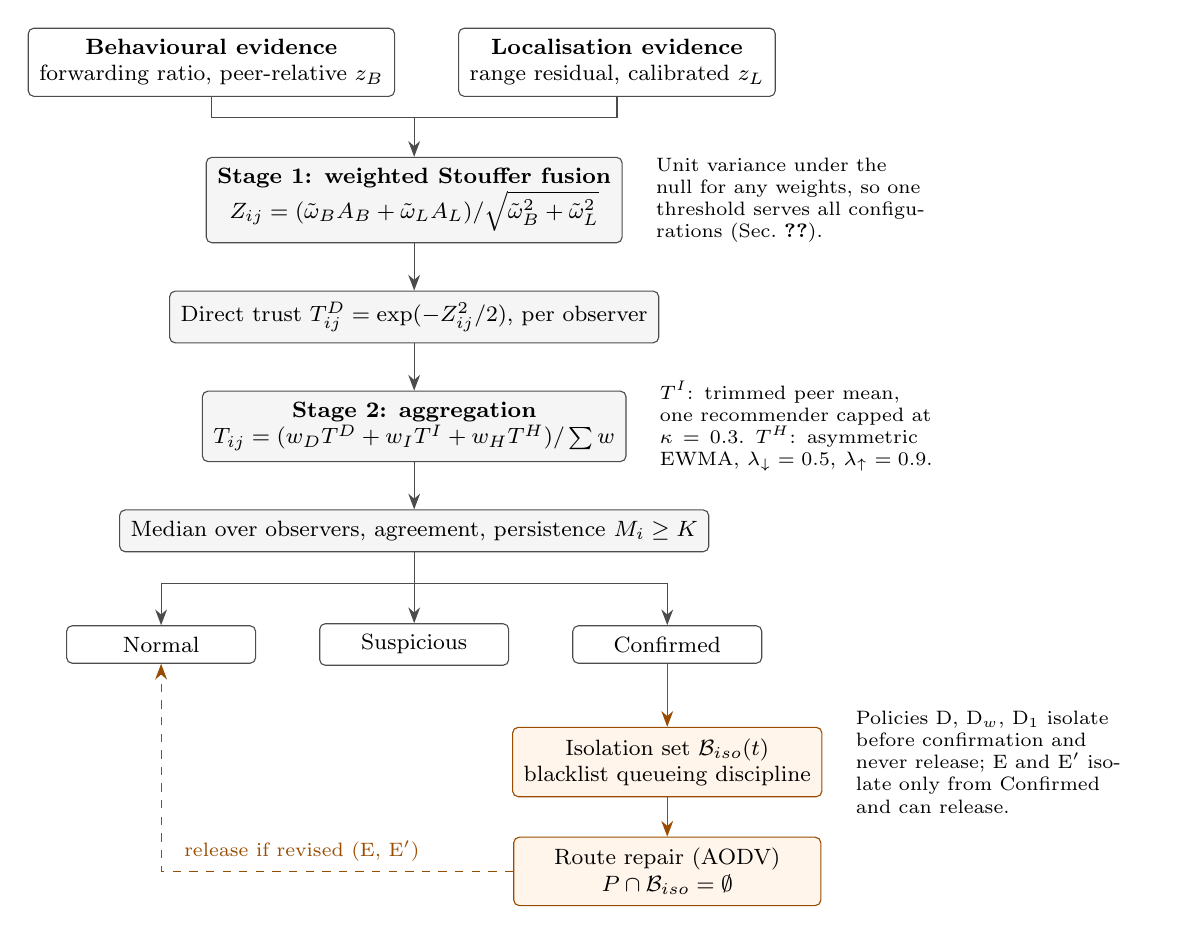
\begin{tikzpicture}[
  font=\footnotesize,
  box/.style={draw=black!70, rounded corners=2pt, align=center, fill=gray!8,
              minimum width=4.6cm, inner sep=4pt},
  ev/.style={box, fill=white, minimum width=3.6cm},
  st/.style={draw=black!70, rounded corners=2pt, minimum width=2.4cm,
             inner sep=4pt, fill=white},
  iso/.style={box, fill=orange!8, draw=orange!60!black, minimum width=3.9cm},
  note/.style={align=left, font=\scriptsize, text width=3.6cm},
  arr/.style={-{Stealth[length=2mm]}, black!70},
  node distance=6mm]
\node[ev] (beh) {\textbf{Behavioural evidence}\\forwarding ratio, peer-relative $z_B$};
\node[ev, right=8mm of beh] (loc) {\textbf{Localisation evidence}\\range residual, calibrated $z_L$};
\node[box, below=12mm of $(beh)!0.5!(loc)$] (s1) {\textbf{Stage 1: weighted Stouffer fusion}\\
  $Z_{ij}=(\tilde\omega_B A_B+\tilde\omega_L A_L)/\sqrt{\tilde\omega_B^2+\tilde\omega_L^2}$};
\node[box, below=of s1] (td) {Direct trust $T^D_{ij}=\exp(-Z_{ij}^2/2)$, per observer};
\node[box, below=of td] (s2) {\textbf{Stage 2: aggregation}\\
  $T_{ij}=(w_D T^D+w_I T^I+w_H T^H)/\sum w$};
\node[box, below=of s2] (dec) {Median over observers, agreement, persistence $M_i \ge K$};
\node[st, below=9mm of dec] (sus) {Suspicious};
\node[st, left=8mm of sus] (nor) {Normal};
\node[st, right=8mm of sus] (con) {Confirmed};
\node[iso, below=8mm of con] (iset) {Isolation set $\mathcal{B}_{iso}(t)$\\blacklist queueing discipline};
\node[iso, below=5mm of iset] (rec) {Route repair (AODV)\\$P \cap \mathcal{B}_{iso} = \emptyset$};
\draw[arr] (beh.south) |- ([yshift=5mm]s1.north) -- (s1.north);
\draw[black!70] (loc.south) |- ([yshift=5mm]s1.north);
\draw[arr] (s1) -- (td);
\draw[arr] (td) -- (s2);
\draw[arr] (s2) -- (dec);
\draw[arr] (dec.south) -- ++(0,-4mm) -| (nor.north);
\draw[arr] (dec.south) -- (sus.north);
\draw[arr] (dec.south) -- ++(0,-4mm) -| (con.north);
\draw[arr, orange!60!black] (con) -- (iset);
\draw[arr, orange!60!black] (iset) -- (rec);
\draw[arr, dashed, orange!60!black] (rec.west) -| node[pos=0.3, above, font=\scriptsize]{release if revised (E, E$'$)} (nor.south);
\node[note, right=3mm of s1] {Unit variance under the null for any weights, so one threshold serves all configurations (Sec.~\ref{sec:calib}).};
\node[note, right=3mm of s2] {$T^I$: trimmed peer mean, one recommender capped at $\kappa=0.3$. $T^H$: asymmetric EWMA, $\lambda_\downarrow=0.5$, $\lambda_\uparrow=0.9$.};
\node[note, right=3mm of iset] {Policies D, D$_w$, D$_1$ isolate before confirmation and never release; E and E$'$ isolate only from Confirmed and can release.};
\end{tikzpicture}}
\caption{Verification pipeline. Behavioural and localisation evidence are
standardised, oriented and fused in Stage~1 to give a per-observer direct
trust value; Stage~2 aggregates that value across observers and over time.
The three-state verdict separates suspicion from confirmation, and the
isolation policies differ only in which evidence authorises removal and
whether removal can be reversed.}
\label{fig:pipeline}
\end{figure}

\subsection{Behavioural evidence}

For beacon $i$ in window $w$, let $P_i^{fwd}$ and $P_i^{recv}$ denote packets
forwarded and received for forwarding. The behavioural observable is the
forwarding ratio
\begin{equation}
\label{eq:fr}
FR_i(t) = \frac{P_i^{fwd}(t)}{P_i^{recv}(t) + \epsilon},
\end{equation}
with $\epsilon$ guarding against division by zero.

We use a single behavioural observable. Composite scores of the form
$w_1 FR_i + w_2(1-DR_i)$ collapse to $(w_1 + w_2) FR_i$, because the drop ratio
is $DR_i = 1 - FR_i$, so they count one observable twice. Genuinely independent
observables, such as routing-response consistency, would each need their own
null calibration and are outside our scope.

The observable is standardised against contemporaneous peers rather than a
static calibrated baseline. Benign congestion depresses forwarding across all
nodes in a neighbourhood simultaneously; measured against a fixed baseline
this registers as individual misbehaviour, whereas measured against peers
observed in the same window a network-wide depression cancels. If
$\mathcal{P}_i$ is the peer set of $i$ with at least $n_{min}$ members,
\begin{equation}
\label{eq:zb}
z_B(w) = \frac{FR_i(w) - \mu(\mathcal{P}_i, w)}{\sigma(\mathcal{P}_i, w) + \epsilon},
\end{equation}
falling back to the static calibrated null where the peer set is too small to
estimate. Equation~\eqref{eq:zb} is the quantity that enters fusion.

\subsection{Localisation evidence}

\subsubsection{Range residual}

The detector is not given the beacon's true position: a node in a MANET has no
such oracle, and a model that consumes one is not implementable. We therefore
score the internal inconsistency of what the beacon broadcasts, which requires
only quantities an observer can measure.

For observer $j$ receiving a beacon from $i$, let $\hat d_{ij}$ be the distance
implied by measured RSSI under the calibrated path-loss model, and
$\tilde d_{ij}$ the distance implied by the coordinates the beacon advertises
together with $j$'s own position estimate. The range residual is
\begin{equation}
\label{eq:resid}
r_{ij}(w) = \bigl| \hat d_{ij}(w) - \tilde d_{ij}(w) \bigr|,
\end{equation}
and the standardised localisation evidence is $r_{ij}$ scored against the
residual null distribution calibrated on clean-network runs,
\begin{equation}
\label{eq:zl}
z_L(w) = \frac{r_{ij}(w) - \mu_r}{\sigma_r + \epsilon}.
\end{equation}
A beacon displaced by $\delta$ inflates $\tilde d_{ij}$ without changing
$\hat d_{ij}$, so $r_{ij}$ grows with $\delta$; an honest beacon leaves $r_{ij}$
at the measurement noise floor. True positions appear in our logs only for
labelling detections as correct or incorrect after the fact.

Two consequences follow. First, the residual is bounded below by RSSI ranging
error, so the attack is undetectable for offsets comparable to that error; the
detection floor is a property of the ranging channel and not of the fusion
rule. Second, an attacker who could also manipulate the RSSI observed by its
neighbours could suppress the residual. Our threat model does not include
physical-layer power manipulation, and we leave it as an open gap.

\subsection{Stage one: evidence fusion}

\subsubsection{Orienting the two evidence streams}

The two standardised statistics point in opposite directions with respect to
misbehaviour. A malicious beacon depresses its forwarding ratio, so $z_B$
becomes large and negative; it inflates its range residual, so $z_L$ becomes
large and positive. Summing the two as they stand would allow a node
misbehaving on both axes to cancel its own evidence. We therefore define a
common one-sided anomaly scale on which larger means more suspicious,
\begin{equation}
\label{eq:orient}
A_B(w) = -z_B(w), \qquad A_L(w) = +z_L(w),
\end{equation}
and all subsequent fusion operates on $A_B$ and $A_L$. The sign convention is
trivial once stated, but Online Resource~1 (Sect.~S3) shows that getting it
wrong produces a detector that fails specifically on hybrid attacks while
continuing to work on single-axis ones.

\subsubsection{Confidence-weighted fusion}

Each branch is weighted by a fixed branch weight and by a confidence factor
saturating in sample count,
\begin{equation}
\label{eq:conf}
c(n) = \frac{n}{n + n_{1/2}},
\end{equation}
with $n_{1/2} = 5$ for localisation and $n_{1/2} = 45$ for behaviour. A single
beacon reception carries positional information directly, whereas forwarding
behaviour is observable only through an accumulation of transit packets. This
asymmetry reappears in the measured confirmation latencies of
Section~\ref{sec:results}. Writing the effective weights as
\begin{equation}
\label{eq:effw}
\tilde\omega_B(w) = \omega_B\, c(n_B(w)), \qquad
\tilde\omega_L(w) = \omega_L\, c(n_L(w)),
\end{equation}
where $n_B$ and $n_L$ are the observation counts available to each branch in
window $w$, the fused statistic is
\begin{equation}
\label{eq:stouffer}
Z_{ij}(w) = \frac{\tilde\omega_B A_B(w) + \tilde\omega_L A_L(w)}
                 {\sqrt{\tilde\omega_B^2 + \tilde\omega_L^2}}.
\end{equation}
A branch with no observations in a window has $c = 0$ and drops out, leaving
the remaining branch unchanged; this is why the confidence factor appears
inside the normalisation.

Direct trust is the fused statistic mapped through the Gaussian kernel
\begin{equation}
\label{eq:phi}
T^D_{ij}(w) = \phi\bigl(Z_{ij}(w)\bigr) = \exp\bigl(-\tfrac12 Z_{ij}(w)^2\bigr),
\end{equation}
so that $T^D = 1$ for a beacon indistinguishable from the calibrated null and
$T^D \to 0$ as the fused statistic moves into either tail. Thresholds on $T^D$
therefore correspond to thresholds on $|Z|$: the values used here,
$\tau_M = 0.40$ and $\tau_N = 0.70$, correspond to $|Z| = 1.354$ and
$|Z| = 0.845$, two-sided null tail probabilities of 0.176 and 0.398.

Two properties of~\eqref{eq:phi} matter. It is even in $Z$, so a deviation in
either direction reduces trust equally; this is deliberate, since a beacon
forwarding implausibly more traffic than its peers is as anomalous as one
forwarding less. Because $\phi$ is applied after fusion rather than before
it, the two-sidedness does not rescue a sign error: it is the fused $Z$ that is
folded, not the individual branches.

\subsubsection{Calibrating the fused statistic}
\label{sec:calib}

The combination rule matters less than how its output is thresholded. Let
$s_B, s_L \in [0,1]$ be evidence scores and $C = \omega_B s_B + \omega_L s_L$
with $\omega_B + \omega_L = 1$. Then
\begin{equation}
\label{eq:convex}
\min(s_B, s_L) \le C \le \max(s_B, s_L),
\end{equation}
so if both scores lie on the benign side of a threshold~$\tau$, so does $C$. A
detector that applies the single-branch threshold to a convex combination
therefore cannot confirm an attacker that both branches miss. Tables built
this way will still show the fused row ahead of the weaker branch, because a
mean of a strong score and a weak one exceeds the weak one; the apparent
advantage comes from the comparison and not from the mechanism.

The bound is a consequence of reusing $\tau$, not of averaging as such. For two
independent standardised branches the arithmetic mean
$\bar z = (z_B + z_L)/2$ has standard deviation $1/\sqrt2$ under the null, so a
threshold recalibrated to the same false-positive rate is $\tau/\sqrt2$, and
the rule $\bar z > \tau/\sqrt2$ is identical to the equal-weight Stouffer rule
$(z_B + z_L)/\sqrt2 > \tau$. What the fusion hypothesis requires is a combined
statistic calibrated against its own null distribution. Weighted Stouffer
combination~\eqref{eq:stouffer} is unit variance under the null whatever the
weights, so a single threshold serves every configuration and the hypothesis
becomes falsifiable: two branches each at $z = 1.5$ combine, with equal
weights, to $Z = 2.12$.

This argument disqualifies uncalibrated combination; it does not make
Stouffer's method the best calibrated rule. Fisher's method, likelihood-ratio
and Bayesian fusion, Dempster--Shafer combination~\cite{singh2020self} and
learned rules can be calibrated in the same sense. We chose Stouffer's method
because it needs no likelihood model for either branch, admits per-branch
weights~\cite{whitlock2005weighted}, and degrades gracefully when one branch
has no observations, which is frequent under mobility. Section~\ref{sec:sweep}
compares it with a disjunctive rule only.

Equation~\eqref{eq:stouffer} assumes $z_B$ and $z_L$ are independent under the
null. In our attack scenarios they are close to independent by construction,
because A1 and A2 disturb disjoint observables. Under a correlated failure,
such as congestion coinciding with a mobility-induced ranging error, the fused
statistic would be optimistic; correcting for it requires an estimated
correlation term.

\subsection{Stage two: trust aggregation}

Direct trust is the Stage~1 output $T^D_{ij}(w)$ of~\eqref{eq:phi}, per
observer and window, with no separate smoothing. It is combined with indirect
and historical trust,
\begin{equation}
\label{eq:combined}
T_{ij}(t) = \frac{w_D T^D_{ij}(t) + w_I T^I_{ij}(t) + w_H T^H_{ij}(t-1)}{w_D + w_I + w_H},
\end{equation}
renormalised over the terms defined in the window. Indirect trust $T^I_{ij}$ is
a trimmed mean (trim fraction 0.2) of the direct trust that observers other
than $j$ hold in $i$, with any single recommender's influence capped at
$\kappa = 0.3$, so that no minority of recommenders can move it
arbitrarily~\cite{liu2008attack}. Historical trust $T^H_{ij}$ is an
exponentially weighted average of past combined trust with asymmetric decay,
$\lambda_\downarrow = 0.5$ when trust falls and $\lambda_\uparrow = 0.9$ when
it rises, so wrongly trusting an attacker costs more than briefly distrusting
an honest node. On a pair's first window $T^H$ is undefined, drops out of the
renormalisation and is seeded from the result; history alone therefore
defines no trust, which constrains the ablation design (Online Resource~1,
Sect.~S6).

\subsection{Confidence, state and confirmation}

Per-observer trust is collapsed to a single per-target confidence by the median
over observers holding a defined opinion in that window,
\begin{equation}
\label{eq:median}
C_i(t) = \operatorname{median}\{\, T_{ij}(t) : j \in O_i(t) \,\},
\end{equation}
where $O_i(t)$ is that observer set and $|O_i(t)| \ge 3$ is required for any
verdict. The median prevents a single observer with an extreme value from
moving the collapsed confidence. The confidence may optionally be smoothed,
$\hat C_i(t) = \gamma C_i(t) + (1-\gamma)\hat C_i(t-1)$, though the evaluated
configuration uses $\gamma = 1$, so temporal memory enters the decision through
the persistence requirement and not through smoothing. The verdict map is
\begin{equation}
\label{eq:verdict}
S_i(t) =
\begin{cases}
\textsc{Normal}, & \hat C_i(t) \ge \tau_N,\\
\textsc{Suspicious}, & \tau_M < \hat C_i(t) < \tau_N,\\
\textsc{Confirmed}, & \hat C_i(t) \le \tau_M,
\end{cases}
\end{equation}
with $0 \le \tau_M < \tau_N \le 1$. Confirmation also requires
persistence,
\begin{equation}
\label{eq:persist}
M_i(t) = \sum_{k=0}^{W-1} \mathbb{I}\bigl[\hat C_i(t-k) \le \tau_M\bigr],
\end{equation}
with $W = K = 3$, so beacon $i$ is confirmed only if the three most recent
windows all satisfy the condition. A verdict also requires agreement: at
least a fraction $a_{min} = 0.5$ of observers holding a defined opinion, and no
fewer than three observers, must place the target below $\tau_M$ in the same
window.

Three further rules complete the decision logic.

\textbf{Single-branch override.} An observer whose direct trust falls below
$\tau_X = 0.10$, corresponding to $|Z| \ge 2.146$, can confirm a target without
satisfying the agreement fraction. An attack visible to only one evidence class
produces one branch far into its tail while the other stays at the null, and
requiring majority agreement there would suppress the detection the
architecture is meant to enable. The override is essential to the coverage
result: under A1 the behavioural branch contributes nothing, and confirmation
proceeds on localisation evidence alone. The A1 and A2 results should be
attributed to fusion together with this override.

\textbf{Asymmetric clearing.} Leaving the confirmed state requires $K_c = 12$
consecutive clean windows against the $K = 3$ required to enter it, a four-fold
asymmetry in the same direction as the trust decay constants. This rule gives
policy E its release behaviour.

\textbf{Evidence-aware release.} Isolation removes a beacon from forwarding, so
while it is isolated its behavioural branch receives too few transit packets
to contribute, and its trust rests on localisation alone. Under policy E a
beacon confirmed on behavioural evidence can therefore be cleared by the
absence of that evidence rather than by its return. Policy E$'$ closes this
path: a beacon confirmed in a window in which behavioural evidence was
available is released only on a clean window in which behavioural evidence is
again available. A beacon confirmed on localisation evidence alone is released
as under E. Section~\ref{sec:release} measures what the rule costs.

\subsection{Isolation}

On confirmation the beacon enters the isolation set, and under a releasing
policy it leaves when released,
\begin{equation}
\label{eq:iso}
\mathcal{B}_{iso}(t) = \bigl(\mathcal{B}_{iso}(t-1) \cup \{\, i : S_i(t) = \textsc{Confirmed} \,\}\bigr)
\setminus \mathcal{R}(t),
\end{equation}
where $\mathcal{R}(t)$ is the set released at $t$ (empty for the policies
that never release). The admissible node set becomes $V'(t) = V \setminus \mathcal{B}_{iso}(t)$.
Every subsequent route must satisfy $P \cap \mathcal{B}_{iso}(t) = \emptyset$.
Enforcement is by a blacklist queueing discipline; route repair is performed by
AODV.

\subsection{Computational and communication cost}
\label{sec:cost}

In each 5\,s step an observer computes one fused statistic per beacon it
hears, so Stage~1 costs $O(|\mathcal{B}|)$ per observer and
$O(N|\mathcal{B}|)$ across the network. Indirect trust is a trimmed mean over
the other observers of a beacon, and the median of~\eqref{eq:median} sorts the
same set, so each beacon costs $O(|O_i| \log |O_i|)$ per window, with
$|O_i| \le N-1$. With three to six monitored beacons and at most 50 nodes,
this is a few hundred arithmetic operations per node per window. A deployment
must also exchange recommendations. If each node broadcasts its direct trust
in every monitored beacon once per step, the network carries $N$ short
messages every 5\,s: 25 in the dense network, against about 600 data packets
in the same interval. In this study the pipeline runs over the simulator's
logged traces, so recommendation messages were not transmitted and their
effect on delivery was not measured.

\subsection{Evaluation quantities}

Recovery time is $T_{rec} = T_{new\text{-}route} - T_{isolation}$, and the
throughput recovery ratio is
\begin{equation}
\label{eq:recov}
R_{TH} = \frac{TH_{after}}{TH_{normal}},
\end{equation}
with $TH$ the delivered throughput; a well-behaved mechanism gives
$R_{TH} \to 1$.

Finally we define a false-isolation cost that we believe is under-reported in
this literature. Let $H$ be the set of honest beacons and $\iota_i(t)$ the
indicator that $i$ is isolated at time $t$. Cumulative false isolation over a
run of duration $T$ is
\begin{equation}
\label{eq:Phi}
\Phi = \int_0^T \sum_{i \in H} \iota_i(t)\, dt,
\end{equation}
in node-seconds. $\Phi$ measures service withdrawn from the network by the
security mechanism itself. A mechanism with a low false-positive rate may
still have large $\Phi$ if it never releases. Because $\Phi$ grows with the
number of honest beacons and with run duration, we also report the
dimensionless form
\begin{equation}
\label{eq:Phibar}
\bar\Phi = \frac{\Phi}{|H| \cdot T},
\end{equation}
the mean fraction of honest-beacon service time withdrawn by the mechanism,
which is comparable across topologies.

\section{Experimental Methodology}
\label{sec:method}

Simulations use ns-3.48~\cite{ns3} with AODV routing over IEEE 802.11.
Network parameters appear in Table~\ref{tab:sim} and detector parameters in
Table~\ref{tab:det}; both were fixed for the entire campaign and no per-scenario
tuning was performed.

\begin{table}[!t]
\caption{Network and simulation parameters.}
\label{tab:sim}
\centering
\footnotesize
\begin{tabular}{@{}ll>{\raggedright\arraybackslash}p{6.4cm}@{}}
\toprule
Parameter & Symbol & Value \\
\midrule
Simulator & -- & ns-3.48 \\
Routing protocol & -- & AODV \\
Field & -- & $500 \times 500$\,m (sparse: $1000 \times 1000$; 50-node: $707 \times 707$) \\
Nodes & $N$ & 25 (50-node campaign: 50) \\
Monitored beacons & $|\mathcal{B}|$ & 3, 1 attacker (50-node campaign: 6, 2 attackers) \\
Transmit power & -- & 30\,dBm \\
Propagation loss model & -- & log-distance \\
Path-loss exponent & $\eta$ & 3.0 \\
Reference loss at 1\,m & $P_0$ & 46.68\,dB \\
Shadowing & $\sigma_{sh}$ & 0\,dB; 4 and 8\,dB in Sec.~\ref{sec:shadow} \\
RSSI measurement noise & $\sigma_{RSSI}$ & 4\,dB \\
Mobility model & -- & random waypoint \\
Node speed & -- & $U(1,5)$\,m/s \\
Pause time & -- & 2.0\,s \\
Traffic & -- & 10 CBR flows, 12\,pkt/s (50-node campaign: 14) \\
Packet size & -- & 512\,B \\
Beacon interval & -- & 1.0\,s \\
PHY data rate & -- & DSSS 1\,Mbps \\
Simulation duration & $T$ & 400\,s \\
Attack start & -- & $t = 30$\,s \\
Per-axis position offset (A1) & $\delta$ & 300\,m \\
Measured mean displacement (A1) & -- & 267\,m \\
Drop probability (A2) & $p$ & 0.6 \\
Hybrid scaling (A3) & -- & $\delta/2$, $p/2$ \\
Runs executed & -- & 780 (Table~\ref{tab:campaign}) \\
\bottomrule
\end{tabular}
\end{table}

\begin{table}[!t]
\caption{Detector parameters. All values fixed across the campaign; none were
tuned per scenario.}
\label{tab:det}
\centering
\footnotesize
\begin{tabular}{@{}llr@{}}
\toprule
Parameter & Symbol & Value \\
\midrule
Observation window / step & -- & 10\,s / 5\,s \\
Branch weights & $\omega_B$, $\omega_L$ & 1.0, 1.0 \\
Confidence half-weight, localisation & $n^L_{1/2}$ & 5 \\
Confidence half-weight, behaviour & $n^B_{1/2}$ & 45 \\
Minimum peer set & $n_{min}$ & 8 \\
Minimum transit packets, behaviour & -- & 5 \\
Trust weights & $w_D$, $w_I$, $w_H$ & 0.5, 0.2, 0.3 \\
Trim fraction / recommender cap & -- / $\kappa$ & 0.2 / 0.3 \\
History decay, falling / rising & $\lambda_\downarrow$ / $\lambda_\uparrow$ & 0.5 / 0.9 \\
Observer agreement & $a_{min}$ & 0.5 \\
Malicious threshold & $\tau_M$ & 0.40 ($|Z| = 1.354$) \\
Normal threshold & $\tau_N$ & 0.70 ($|Z| = 0.845$) \\
Persistence / clearing persistence & $K$ / $K_c$ & 3 / 12 windows \\
Minimum observers & -- & 3 \\
Single-branch override & $\tau_X$ & 0.10 ($|Z| = 2.146$) \\
Bounded transform & $\phi$ & $\exp(-Z^2/2)$, Eq.~\eqref{eq:phi} \\
\bottomrule
\end{tabular}
\end{table}

Two properties of the radio configuration bound what the localisation branch
is asked to do. First, the primary campaign disables shadowing, so the channel
is deterministic log-distance path loss and the only stochasticity entering
the localisation branch is the 4\,dB measurement noise added at the receiver.
A real deployment would add multipath, obstruction and correlated shadowing,
all of which inflate the range residual for honest beacons and raise the
detection floor; Section~\ref{sec:shadow} repeats the campaign at
$\sigma_{sh} = 4$ and 8\,dB. Second, the observer inverts distance from
measured RSSI using the same path-loss parameters,
\begin{equation}
\label{eq:dhat}
\hat d_{ij} = 10^{(P_{tx} - P_0 - \mathrm{RSSI}_{ij})/(10\eta)},
\end{equation}
so $\hat d_{ij}$ in~\eqref{eq:resid} is derived entirely from a quantity the
observer measures. No true position enters the detector.

The full-intensity attack magnitudes are large. A position offset of
$\delta = 300$\,m in a $500 \times 500$\,m field is a very large lie, and a
drop probability of $p = 0.6$ is an aggressive grey hole. Both were chosen to
establish the mechanism, and they do not represent a realistic adversary;
Section~\ref{sec:sweep} sweeps the hybrid attack down to a displacement of
3.75\,m and a drop probability of 0.75\%.

\begin{table}[!t]
\caption{Simulation campaign. Calibration seeds are clean runs held out from
testing. Of the first 570 runs, 45 repeat a configuration and seed run
elsewhere in the campaign and reproduced it byte for byte; closed-loop rounds
that re-enforce an unchanged schedule likewise repeat their predecessor.}
\label{tab:campaign}
\centering
\footnotesize
\begin{tabular}{@{}p{3.3cm}p{6.6cm}r@{}}
\toprule
Part & Design & Runs \\
\midrule
Original campaign & 4 scenarios $\times$ 5 seeds (detection) and 3 attacks
$\times$ 3 policies $\times$ 5 seeds with isolation enforced in the simulator & 65 \\
30-seed campaign & 4 scenarios $\times$ seeds 1--30, plus calibration seeds
101--105 & 125 \\
Intensity sweep, primary & A3, 11 levels $\times$ 10 seeds, drop $= 0.3f$ & 110 \\
Intensity sweep, second pairing & A3, 8 levels $\times$ 10 seeds, drop $= 0.15f$ & 80 \\
Shadowing & $\sigma_{sh} \in \{4, 8\}$\,dB, 4 scenarios $\times$ 20 seeds, plus
5 calibration seeds each & 170 \\
Clean enforced replay & policies D$_1$, E on clean seeds 1--10, schedules
from the replay enforced in the simulator & 20 \\
Iterated closed loop & policies E, E$'$ $\times$ \{A2, clean\} $\times$ seeds
1--10 $\times$ 3 rounds & 120 \\
Sparse topology & 25 nodes in $1000 \times 1000$\,m, 4 scenarios $\times$ 10
seeds, plus 5 calibration seeds & 45 \\
50-node network & 50 nodes in $707 \times 707$\,m, 6 monitored beacons, 2
attackers, 4 scenarios $\times$ 10 seeds, plus 5 calibration seeds & 45 \\
\midrule
Total & & 780 \\
\bottomrule
\end{tabular}
\end{table}

The sparse campaign keeps every parameter of Table~\ref{tab:sim} but
quadruples the field area, so that nodes have about a quarter as many
neighbours and routes are longer and break more often; detector thresholds
are recalibrated on its own clean seeds. The 50-node campaign keeps node
density constant: twice the nodes in twice the area, six monitored beacons of
which two attack, and 14 traffic flows. Its thresholds are likewise
recalibrated on its own clean seeds.

Table~\ref{tab:campaign} lists the campaign. Three groups of runs repeat
another part of it (the enforced runs' control arm, the original detection
runs, and the primary sweep's full-intensity level); every repeated run
reproduced its counterpart byte for byte, as did a run repeated on a second
machine with a separately built simulator, and no analysis uses the same
simulation twice. Throughput recovery, mechanism accounting, localisation
error and the aggregation ablation come from the original campaign, in which
isolation is enforced by the simulator. Coverage, latency, false positives and
$\Phi$ come from the 30-seed campaign, in which each isolation policy is
replayed offline over the same per-window verdict stream, so every policy's
$\Phi$ is paired by seed. The replay assumes that an isolation does not alter
later verdicts. For D, D$_w$ and D$_1$, which never release, a beacon's first
isolation time is computed exactly from verdicts issued before any isolation;
E's release times depend on verdicts issued while another beacon may be
isolated, whose load shifts onto its neighbours. We therefore enforced the
replayed D$_1$ and E schedules on clean seeds 1--10, re-verified the enforced
traces with the same calibration and rebuilt each schedule from the verdicts
produced under isolation (20 runs, Section~\ref{sec:phi}), and iterated this
loop for three rounds for E and E$'$ on the A2 and clean scenarios
(Section~\ref{sec:release}). We compare six isolation policies:

\begin{itemize}
\item \textbf{C, no isolation.} Control.
\item \textbf{D, immediate isolation.} Isolate on the first Suspicious or
      Confirmed window; never release.
\item \textbf{D$_w$, warm-up guard.} As D, but a beacon's first three usable
      windows, counted from its own first usable window, cannot trigger
      isolation.
\item \textbf{D$_1$, single malicious window.} Isolate on the first window in
      which confidence falls below $\tau_M$ with enough observers in
      agreement, without persistence; never release. This is the strongest
      immediate-isolation policy.
\item \textbf{E, confirmation-gated isolation.} Isolate on confirmation;
      release when the verdict is revised.
\item \textbf{E$'$, evidence-aware release.} As E, but a beacon confirmed while
      behavioural evidence was available is released only when that evidence
      returns (Section~\ref{sec:framework}). E$'$ was introduced after the
      enforced runs showed that E re-admits forwarding attackers
      (Section~\ref{sec:release}).
\end{itemize}

Policies D, D$_w$ and D$_1$ are constructions for comparison, not models of a
published method; in particular they are not EMBN-MANET, whose response acts
on localisation coordination rather than forwarding. Isolation is enforced by
a blacklist queueing discipline on every node, including in control runs;
with an empty blacklist it behaves as a plain FIFO.

\subsection{Literature baselines}
\label{sec:baselinedef}

Two baselines re-implement the evidence class and decision rule of a
well-known design and run on the same traces as our pipeline. They are not
reimplementations of complete published systems.

\textbf{LND, localisation-only alert counting.} After Liu, Ning and
Du~\cite{liu2005detecting}, the evidence class EMBN-MANET also uses. In each
window an observer with at least three receptions raises an alert against a
beacon whose mean range residual exceeds $\rho$, and the beacon is revoked
permanently once more than $\tau'$ alerts have accumulated.

\textbf{WD, behaviour-only reputation.} After the watchdog of Marti
et al.~\cite{marti2000mitigating} and the Beta reputation of
CONFIDANT~\cite{buchegger2002confidant}. A beacon's reputation is the mean of
a Beta distribution whose parameters are the counts of forwarded and
unforwarded transit packets, faded by 0.9 per 10\,s window; once at least 20
packets of evidence have accumulated, the beacon is isolated permanently when
its reputation falls below $\tau_W$.

\textbf{LND+WD.} Both detectors run side by side and a beacon is isolated
when either fires. This is the disjunctive rule of Section~\ref{sec:sweep}
applied to two independently designed detectors.

All three thresholds come from the held-out clean calibration seeds of each
channel and from nothing else: $\rho$ is the 99th percentile of clean
residuals, $\tau_W$ the 1st percentile of clean reputations, and $\tau'$ the
smallest alert count at which no calibration run revokes any beacon. At
0, 4 and 8\,dB this gives $\rho = 63$, 87 and 170\,m, $\tau_W = 0.81$, 0.57
and 0.38, and $\tau' = 10$, 11 and 15. A sweep of $\tau'$ on the test runs,
reported for transparency, shows the trade-off the calibration resolves: at
$\tau' = 5$ LND revoked 31 of 90 honest node-seeds on the clean network, at
10 three, and at 20 none, while still revoking the A1 attacker in every seed.

\subsection{Reproducibility}

The simulator is ns-3.48 built with GCC on Ubuntu under WSL2, with the analysis
pipeline in Python~3. Runs were executed on a laptop with 8\,GB of memory. Simulator sources, the analysis pipeline and the scripts
for every campaign are public at
\url{https://github.com/kraghu356/manet-beacon-trust}. Every run uses an explicit integer seed, so any run is
reproducible from its scenario, policy and seed. Detection thresholds were
fixed on the trust scale before any attack scenario was run, and the null
distributions of $A_B$ and $A_L$ were calibrated on clean-network runs that
are never used for testing: seeds 101--105 for the 30-seed and shadowing
campaigns, recalibrated per channel. No threshold was chosen by reference to a
result reported in this paper. Several simulator parameters are supplied at
invocation instead of being compiled in, so the released command lines
define the experiment and the source defaults do not. Statistical intervals are percentile
bootstrap intervals over seeds (10{,}000 resamples), paired across policies
where policies share seeds. An AI assistant (Claude, Anthropic) helped write
parts of the analysis code; the authors reviewed and tested that code, and
every reported number is regenerated by the released scripts.

\section{Results}
\label{sec:results}

\subsection{Evidence coverage}
\label{sec:coverage}

\begin{table}[!t]
\caption{Attacker confirmation by evidence configuration, 30 seeds per cell.}
\label{tab:coverage}
\centering
\footnotesize
\begin{tabular}{@{}lccc@{}}
\toprule
Configuration & A1 & A2 & A3 \\
\midrule
Behavioural only & 3/30 & 30/30 & 30/30 \\
Localisation only & 30/30 & 0/30 & 30/30 \\
Fused & 30/30 & 30/30 & 30/30 \\
\bottomrule
\end{tabular}
\end{table}

Table~\ref{tab:coverage} reports attacker
confirmation by evidence configuration. The inversion between the two
single-evidence rows admits a structural explanation. Under A1 the attacker
forwards honestly, so no behavioural quantity departs from its null
distribution. The delivered-throughput series of every A1 run is identical to
the clean-network run of the same seed, in all 30 seeds (Online Resource~1, Fig.~S2).
Behavioural evidence alone nevertheless confirmed the A1 attacker in 3 of 30
seeds. These confirmations carry no attack signal: on the clean network the
behavioural branch alone confirms honest beacons in 15 of 90 node-seeds (17\%),
a higher rate than its 10\% on the A1 attacker. Symmetrically, under A2 the
attacker advertises its true position, and localisation evidence alone
confirmed it in 0 of 30 seeds; it confirmed no honest beacon in any run of the
campaign.

A single-evidence detector therefore has a region of the attack space it
cannot observe, and an adversary who knows which evidence is collected may
choose to occupy it. This follows from what each evidence class can physically
observe, and no threshold setting changes it.

The scope of the claim is narrow. Table~\ref{tab:coverage} establishes that
collecting both classes covers both attacks. It does not establish that
Stouffer fusion is responsible: a disjunctive rule that thresholds each branch
independently and confirms on either would achieve the same result on A1 and
A2, because in each case one branch is far into its tail while the other is
silent. Fusion and disjunction separate only where both branches are weak
simultaneously. The coverage result is a result about evidence collection; the
fusion-rule question is taken up in Section~\ref{sec:sweep}.

Two timing quantities are reported and must not be conflated. Detection
latency is the interval between attack onset and the first window in which the
attacker is confirmed. Isolation time is the timestamp of the first isolate
event written to the enforcement schedule. Over 30 seeds, the fused pipeline
confirmed the attacker in every seed of every attack. Median latency was
15.0\,s for A1 and A3 and 27.5\,s for A2 (means 20.0, 20.7 and 41.7\,s), with
a tail of slower confirmations reaching 80, 75 and 160\,s respectively.

The difference between attack classes is a property of the evidence, and the
model predicts its direction. Behavioural evidence reaches half confidence
weight at $n_{1/2} = 45$ observations against 5 for localisation
\eqref{eq:conf}. A2 is observable only through the behavioural branch, so its
confidence factor climbs an order of magnitude more slowly and confirmation
waits on the accumulation of transit packets. A1 and A3 are observable through
localisation, for which a handful of beacon receptions suffice. The constants were
fixed during calibration and not adjusted afterwards.

\subsection{Attack intensity and the fusion region}
\label{sec:region}

All three configurations confirm the A3 attacker in every seed, so the
experiment designed to show a fusion sensitivity advantage did not show one.
To locate where an advantage could appear we assume that branch anomaly
magnitude scales approximately linearly with attack intensity,
$A(f) \approx f A(1)$. For an RSSI-derived range residual under mobility, and
for a drop-rate statistic estimated from a finite window, that linearity is
plausible over a limited range but not guaranteed, so what follows locates the
region under an idealised model of the detector.

Let $\theta_B$ and $\theta_L$ be the intensities at which each branch alone
reaches the decision threshold, so that branch $X$ has anomaly
$\theta f/\theta_X$ at intensity $f$. With effective weights
$\tilde\omega_B, \tilde\omega_L$ the fused statistic of~\eqref{eq:stouffer}
crosses the threshold at
\begin{equation}
\label{eq:ffused}
f_F = \frac{\sqrt{\tilde\omega_B^{2} + \tilde\omega_L^{2}}}
           {\tilde\omega_B/\theta_B + \tilde\omega_L/\theta_L},
\end{equation}
and the family passes through a fusion-only region (an intensity at which
fusion confirms and neither branch does) precisely when
\begin{equation}
\label{eq:region}
f_F < \min(\theta_B, \theta_L).
\end{equation}
When the branches are equally sensitive the region is
$\theta_B/\sqrt2 < f < \theta_B$: a factor of $\sqrt2$ in intensity, half an
octave, and the widest it can be. Writing
$r = \max(\theta_B,\theta_L)/\min(\theta_B,\theta_L)$ for the sensitivity
ratio, \eqref{eq:region} with equal effective weights reduces to
\begin{equation}
\label{eq:ratio}
\frac{\sqrt{2}\,r}{1+r} < 1
\quad\Longleftrightarrow\quad
r < 1 + \sqrt{2} \approx 2.414 .
\end{equation}
With unequal weights, let $\tilde\omega_s$ weight the more sensitive branch and
$\tilde\omega_w$ the less sensitive one; the region exists if and only if
$r < \tilde\omega_w / \bigl(\sqrt{\tilde\omega_s^2 + \tilde\omega_w^2} -
\tilde\omega_s\bigr)$, which falls below $1+\sqrt{2}$ when the less sensitive
branch carries more weight (1.618 at twice the weight).

The condition concerns the attack family, not the detector. In units of the
decision threshold, $u = A_L/\theta$ and $v = A_B/\theta$, a branch confirms
alone when its coordinate reaches 1, and with equal weights the fused
statistic confirms when $u + v \ge \sqrt2$, so the fusion-only region is the
triangle
\begin{equation}
\label{eq:wedge}
u < 1, \qquad v < 1, \qquad u + v > \sqrt2,
\end{equation}
which is non-empty for every Stouffer detector with positive weights. Scaling
an attack by intensity $f$ moves it along the ray
$(u, v) = f\,(1/\theta_L, 1/\theta_B)$, and~\eqref{eq:ratio} is the condition
for that ray to cross the triangle. A lopsided attack crosses the more
sensitive branch's threshold first and misses the region. The ratio $r$ can be
read from single-branch detection curves before any fusion experiment;
Section~\ref{sec:sweep} tests it on two families that differ only in their
mix.

\subsection{False positives}
\label{sec:fp}

Over the 30-seed campaign the fused pipeline confirmed 9 of 90 honest
node-seeds on the clean network (10\%, Wilson 95\% interval 5.4--17.9\%) and 21
of 180 under attack (11.7\%, 7.8--17.2\%). The behavioural branch alone
confirmed 15 of 90 on the clean network and 35 of 180 under attack; the
localisation branch alone confirmed none. False confirmations are therefore a
property of the behavioural branch, whose peer-relative score fires whenever a
beacon's forwarding departs from its contemporaneous neighbours for benign
reasons such as mobility. Fusion with a silent localisation branch damps
these confirmations without removing them. With three monitored beacons per run, one false
positive moves per-run accuracy by 33 percentage points, which is why we
report counts instead of accuracy.

\subsection{Attack-intensity sweeps}
\label{sec:sweep}

We tested the fusion condition directly with two sweeps of the hybrid attack.
The primary sweep scales displacement and drop probability together from the
full-intensity A3 configuration over eleven levels, ten seeds each (110 runs,
Online Resource~1, Table~S1). The second repeats eight levels with the drop
probability halved relative to displacement (80 runs, Table~S2).
Fig.~\ref{fig:sweep} shows both.

\begin{figure}[!t]
\centering
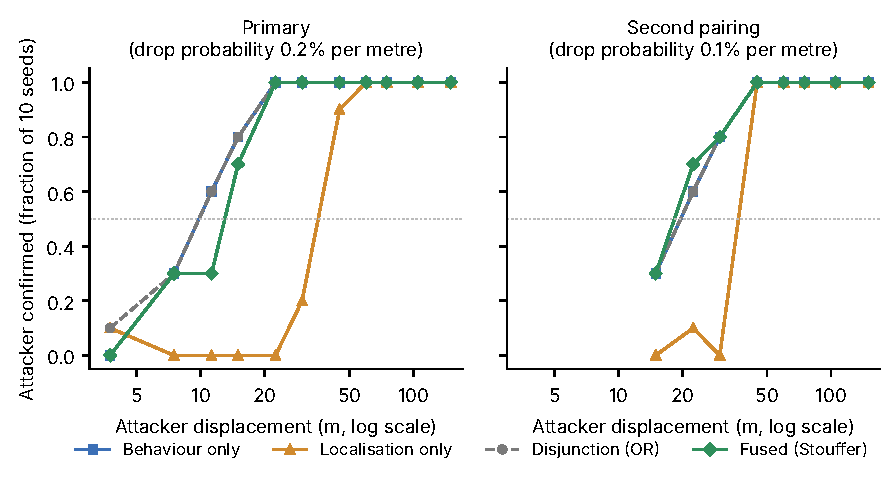
\includegraphics[width=\textwidth]{fig4_sweep}
\caption{Attacker detection across the two intensity sweeps, ten seeds per
point. Left: the branches' 50\% thresholds lie a factor of 3.63 apart, beyond the
$1+\sqrt2$ bound, and fusion falls below the disjunctive rule near the
behavioural threshold. Right: halving the drop rate moves the behavioural
curve and brings the ratio to 1.87, inside the bound, and fusion matches or
exceeds disjunction.}
\label{fig:sweep}
\end{figure}

\subsubsection{Primary sweep: the attack path misses the fusion-only region}

Behavioural detection falls from 8 of 10 at 15\,m to 6, 3 and 0 of 10 at 11.25,
7.5 and 3.75\,m; it reaches half detection at $\theta_B = 9.8$\,m, interpolated
on log intensity. Localisation evidence reaches half detection at
$\theta_L = 35.7$\,m. The measured ratio is $r = 3.63$. Resampling each level's
ten seeds as independent Bernoulli trials gives a bootstrap 95\% interval of
[2.67, 5.47], and fewer than 0.5\% of resamples fall below $1+\sqrt2$. Since
the less sensitive branch, localisation, carries the larger effective weight
through~\eqref{eq:conf}, the applicable bound is tighter still. This attack
family's path does not enter the fusion-only region.

The sweep shows the consequence the bound predicts. Where the behavioural
branch is near its threshold, adding the weaker localisation branch dilutes
it: at 11.25\,m fusion confirmed the attacker in 3 of 10 seeds against 6 for
the disjunctive rule, and at 15\,m in 7 against 8; at every stronger intensity
both confirmed it in all ten. The mechanism is visible at seed level. Where the
behavioural branch is anomalous and the localisation branch sits at its null,
equal-weight Stouffer combination computes $(A_B + 0)/\sqrt2$, attenuating a
live branch by 29\%, because a branch with adequate sample count carries
confidence weight whether or not it carries signal. Disjunction is immune,
since it never mixes the two. The same attenuation works in the opposite
direction for honest beacons: a benign behavioural deviation that would cross
the threshold alone is also scaled by $1/\sqrt2$ when the localisation branch
is at its null. Equal-weight fusion therefore trades sensitivity near the
threshold for suppression of single-branch false alarms. Sections~\ref{sec:fp},
\ref{sec:sparse} and~\ref{sec:scale} measure the second side of that trade.

\subsubsection{Second pairing: the condition predicts the outcome}

The ratio depends on how the sweep couples the two intensities, and the second
sweep tests whether~\eqref{eq:ratio} predicts the consequence. The behavioural
curve moved exactly as drop probability dictates: 3, 6 and 8 of 10 at drops of
1.5, 2.25 and 3\% in both sweeps, so behavioural detection depends on the drop
rate alone. Localisation, which depends on displacement alone, stayed close
to its primary-sweep value, at $\theta_L = 36.7$\,m. With $\theta_B = 19.7$\,m the ratio falls to $r = 1.87$
(bootstrap 95\% interval [1.41, 2.21]), inside the equal-weight bound in every
resample.

The outcome changed as the condition predicts. Fusion never confirmed fewer
attackers than the disjunctive rule. At $f = 0.15$, at which the behavioural
branch alone confirmed 6 of 10, fusion confirmed 7: one seed in which neither
branch crossed its threshold but their combined evidence did. One seed is weak
evidence and we do not report it as a fusion benefit. What the two sweeps
establish is that the same detector dilutes or helps depending on how the
attack family mixes its two misbehaviours, and that the ratio predicting which
can be measured before fusion is applied. The effective weights vary by window
through~\eqref{eq:conf}; if localisation carries twice the weight of behaviour,
the bound tightens to 1.618, which 17\% of resamples satisfy.

Taken together with Table~\ref{tab:coverage}, the finding is that evidence
collection determines coverage, and whether the combination rule adds anything
against a given attack family is decided by the branches' relative
sensitivity to that family.

\subsection{Comparison with literature baselines}
\label{sec:baselines}

Table~\ref{tab:baselines} compares the pipeline with the baselines of
Section~\ref{sec:baselinedef} on identical traces. The pipeline's false
isolation is that of policy E$'$, since the baselines also isolate on their
own detection and, like E$'$ in practice, do not release.

\begin{table}[!t]
\caption{Pipeline against literature baselines on identical traces. Detection
counts the attacker isolated after onset; FI is honest beacons isolated on the
clean network; $\bar\Phi$ is clean-network false isolation (E$'$ for the
pipeline); latency is the median time from onset to isolation, in seconds,
for A1 / A2 / A3, given only where the attacker was detected in at least half
the seeds. 30 seeds at 0\,dB and 20 under shadowing.}
\label{tab:baselines}
\centering
\footnotesize
\setlength{\tabcolsep}{3.5pt}
\begin{tabular}{@{}llcccccc@{}}
\toprule
$\sigma_{sh}$ & Method & A1 & A2 & A3 & FI & $\bar\Phi$ & Latency A1 / A2 / A3 \\
\midrule
0\,dB & LND & 30/30 & 2/30 & 30/30 & 3/90 & 0.003 & 10 / -- / 15 \\
      & WD & 1/30 & 30/30 & 30/30 & 4/90 & 0.031 & -- / 20 / 40 \\
      & LND+WD & 30/30 & 30/30 & 30/30 & 7/90 & 0.034 & 10 / 20 / 15 \\
      & Pipeline & 30/30 & 30/30 & 30/30 & 9/90 & 0.050 & 15 / 27.5 / 15 \\
4\,dB & LND & 20/20 & 1/20 & 20/20 & 2/60 & 0.005 & 15 / -- / 22.5 \\
      & WD & 4/20 & 20/20 & 13/20 & 7/60 & 0.050 & -- / 60 / 270 \\
      & LND+WD & 20/20 & 20/20 & 20/20 & 8/60 & 0.054 & 15 / 60 / 22.5 \\
      & Pipeline & 20/20 & 20/20 & 20/20 & 6/60 & 0.045 & 15 / 125 / 20 \\
8\,dB & LND & 20/20 & 0/20 & 20/20 & 1/60 & 0.000 & 20 / -- / 65 \\
      & WD & 0/20 & 20/20 & 3/20 & 0/60 & 0.000 & -- / 120 / -- \\
      & LND+WD & 20/20 & 20/20 & 20/20 & 1/60 & 0.000 & 20 / 120 / 65 \\
      & Pipeline & 20/20 & 20/20 & 19/20 & 0/60 & 0.000 & 22.5 / 150 / 155 \\
\bottomrule
\end{tabular}
\end{table}

The single-evidence baselines reproduce the coverage result with detectors
we did not design. The localisation-only detector revoked the A1 and A3
attackers in every seed of every channel and the A2 attacker in at most 2 of
30, and those few revocations came at least 225\,s after onset, at about the
rate at which it revoked honest beacons. The behaviour-only detector isolated
the A2 attacker in every seed and the A1 attacker in at most 4 of 20. Each
literature family is blind to the attack outside its evidence class, as
Table~\ref{tab:families} predicts from published descriptions.

The disjunction of the two baselines is the more instructive comparison, and
on it the pipeline does not win. LND+WD covered every attack in every channel
with false isolation statistically indistinguishable from the pipeline's: the
paired difference in clean-network $\Phi$ (pipeline minus LND+WD) was 19
node-seconds at 0\,dB (95\% CI $[-22, 61]$) and $-10$ at 4\,dB ($[-62, 43]$),
and both were zero at 8\,dB. It isolated attackers as fast or faster. The
pipeline was slower by a mean of 3.7\,s on A1 at 0\,dB (CI $[2.0, 5.2]$), by
60\,s on A2 at 4\,dB ($[18, 104]$) and by 77\,s on A3 at 8\,dB ($[33, 122]$),
and no paired interval showed it faster.

This is what Section~\ref{sec:region} predicts. A1 and A2 each disturb one
branch only, and A3 at its evaluated intensity lies above both branches'
individual thresholds rather than in the fusion-only region, so for every
attack evaluated here a disjunction loses nothing to fusion and
avoids the attenuation of a live branch by a silent one. The latency gap is
largest under shadowing, plausibly because the pipeline's behavioural branch
also waits for its confidence weight to saturate, which a reputation
threshold does not. In this network, therefore, the pipeline's detection is
matched by two calibrated classical detectors run in parallel.
Sections~\ref{sec:sparse} and~\ref{sec:scale} show that this does not carry
over to a sparse or a larger network; there the same disjunction withdrew
11--24\% of honest-beacon service against 0--3\% for the pipeline.

\subsection{Isolation policy under attack}
\label{sec:policy}

Table~\ref{tab:policy} reports the enforced runs of
the original campaign, five seeds per cell, and Online Resource~1 (Figs.~S3 and S4)
shows the recovery intervals and the time
of first isolation under each policy over the 30-seed campaign. Detection is
identical across policies within each attack: the policies differ only in what
follows a verdict.

\begin{table}[!t]
\caption{Isolation policy comparison in the enforced runs, five seeds per cell.
Times in seconds, means over seeds; the attack begins at $t = 30$\,s. Policy C performs no
isolation.}
\label{tab:policy}
\centering
\footnotesize
\begin{tabular}{@{}llccc@{}}
\toprule
Attack & Policy & Isolation time & $R_{TH}$ & Recovery time \\
\midrule
A1 & C & -- & 0.97 & -- \\
   & D & 20.0 & 0.92 & 5.2 \\
   & E & 45.0 & 0.95 & 44.8 \\
A2 & C & -- & 0.93 & -- \\
   & D & 20.0 & 0.94 & 6.2 \\
   & E & 54.0 & 0.90 & 25.6 \\
A3 & C & -- & 0.93 & -- \\
   & D & 20.0 & 0.95 & 4.2 \\
   & E & 45.0 & 0.94 & 35.0 \\
\bottomrule
\end{tabular}
\end{table}

Policy D first isolates at a median of 15\,s in every scenario, including the
clean network, before the attack begins at 30\,s, so what it removes cannot be
the attacker and its fast recovery time of 4.2--6.2\,s is an artefact. The
20.0\,s in Table~\ref{tab:policy} is a five-seed mean (seeds 10--35\,s) under
the original campaign's calibration. D$_w$ and D$_1$ first isolate at medians
of 30 and 35\,s. Policy E first isolates at a median of 45\,s under A1 and A3
and 57.5\,s under A2, which is 30\,s plus the detection latency.

Recovery ratios span 0.90--0.97 across all nine cells, with confidence
intervals far wider than the differences between them, so we claim no
throughput advantage for any policy. Throughput debt, intended as a summary
recovery metric, returned non-zero values on clean runs because the baseline
window is short relative to throughput variance, and is not used.

\subsection{Cumulative false isolation}
\label{sec:phi}

The comparison that separates the policies is not made under attack. On a clean
network every isolation is a false isolation, and $\Phi$ from~\eqref{eq:Phi} is
directly measurable. Table~\ref{tab:phivariants} reports
it over 30 seeds for every policy, on the clean network and under each attack.

\begin{table}[!t]
\caption{Cumulative false isolation $\Phi$ (node-seconds) of honest beacons by
policy, 30 seeds. Honest isolated counts node-seeds; 95\% intervals are
percentile bootstrap over seeds. The final column is the paired difference from
policy E.}
\label{tab:phivariants}
\centering
\footnotesize
\setlength{\tabcolsep}{4pt}
\begin{tabular}{@{}llcrcc@{}}
\toprule
Network & Policy & Honest isolated & $\Phi$ & 95\% CI & $\Phi - \Phi_E$ [95\% CI] \\
\midrule
Clean & D     & 90/90 & 1052 & [1025, 1077] & 1005 [964, 1044] \\
      & D$_w$ & 90/90 & 1018 & [994, 1039]  & 971 [933, 1006] \\
      & D$_1$ & 88/90 & 897  & [843, 950]   & 851 [785, 911] \\
      & E     & 9/90  & 47   & [18, 79]     & -- \\
A1    & D$_1$ & 59/60 & 611  & [573, 648]   & 565 [519, 609] \\
      & E     & 8/60  & 47   & [18, 79]     & -- \\
A2    & D$_1$ & 58/60 & 587  & [532, 638]   & 557 [499, 612] \\
      & E     & 7/60  & 30   & [10, 54]     & -- \\
A3    & D$_1$ & 59/60 & 586  & [526, 639]   & 571 [514, 625] \\
      & E     & 6/60  & 15   & [2, 31]      & -- \\
\bottomrule
\end{tabular}
\end{table}

Policy D isolates on the first suspicious window, which typically falls before
any attacker is active. To test whether the comparison rests on this start-up
transient, D$_w$ ignores each beacon's first three usable windows and D$_1$
isolates on the first window of malicious evidence without persistence. On the
clean network D$_w$ isolated all 90 honest node-seeds and D$_1$ 88, with mean
$\Phi$ of 1018 and 897 node-seconds against 47 for E, which isolated 9. The
paired difference between D$_1$ and E is 851 node-seconds (95\% CI
[785, 911]); D$_1$ withdraws 74.8\% of honest-beacon service and E 3.9\%.
Removing the persistence requirement alone is therefore enough to isolate
nearly every honest beacon, and under attack every paired interval also
excludes zero.

The replay itself was tested on clean seeds 1--10 by enforcing the replayed
schedules and rebuilding them from the verdicts issued under isolation
(Section~\ref{sec:method}). Isolation lowered $\Phi$ for both policies: D$_1$
from 910.5 to 829.5 node-seconds (paired difference $-81$, 95\% CI
$[-201.5, 45.5]$) and E from 32.5 to 24.5 (difference $-8$, CI $[-22, 0]$).
Neither interval excludes zero, and per seed the D$_1$ difference ranged from
$-370$ to $+295$, so the replay is unbiased within this resolution but noisy
for the immediate policy, and per-seed values of $\Phi$ for D$_1$ should not
be read individually. The comparison the paper rests on survived: under
isolation D$_1$ withdrew 69.1\% of honest-beacon service and E 2.0\%, D$_1$
exceeded E in all ten seeds, and the paired difference was 805 node-seconds
(CI $[693.5, 917]$) against 878 in the replay. For E the replay, if anything,
overstates $\Phi$.

The mechanism is that the policies inherit different bounds. Policy E isolates
only on confirmation, so its false-isolation rate is bounded by the detector's
false-confirmation rate of about 10\% (Section~\ref{sec:fp}). The immediate
policies isolate on weaker evidence, which on an uncontested network fires on
nearly every monitored beacon. The three-state verdict's contribution is the
tighter bound; it does not change what the detector can see.
Section~\ref{sec:release} shows that release contributes little to the gap.

The immediate policies are our own constructions. Published schemes usually
wait for evidence to accumulate: the localisation-only baseline revokes only
after more than $\tau'$ alerts and the behaviour-only baseline only after 20
packets, and both had low false isolation in the dense network (0.3\% and
3.1\%, Table~\ref{tab:baselines}). Table~\ref{tab:phivariants} therefore
measures what acting before evidence accumulates costs (about 75\% of
honest-beacon service), not a comparison with published practice.

\subsection{Release under isolation}
\label{sec:release}

The schedules above were built from verdicts issued while no beacon was
isolated. Re-verifying the enforced runs of the original campaign exposed a
behaviour that this construction hides. While a beacon is isolated it
forwards no transit traffic, so its behavioural branch falls below the
minimum sample: across the enforced runs behavioural evidence was usable in
1.6\% of the windows in which a beacon was isolated, against 54\% for the same
beacons and windows without isolation, while localisation evidence remained
usable in every window. For the A2 attacker, whose only signature is
behavioural, the fused trust therefore recovers once it is isolated. When the
E schedule was rebuilt from the verdicts issued under isolation, the A2
attacker was isolated at 45--65\,s and released at 115--160\,s in all five
seeds, after the twelve clean windows that clearing requires. A1 and A3
remained isolated, because their position lie keeps the localisation branch
in its tail. In a closed loop E would therefore cycle a forwarding attacker
between isolation and re-admission. Unlike timed redemption or an on--off
attack~\cite{bansal2003ocean,sun2006attacks}, this needs no timer and no
change in the attacker's behaviour. The replayed schedules contain milder
cases of the same effect: even without isolation, E released the attacker in
7 of the 90 attacked runs of the 30-seed campaign and in 3 of 60 at 4\,dB.

Policy E$'$ (Section~\ref{sec:framework}) releases a beacon confirmed on
behavioural evidence only when that evidence returns, which an isolated
beacon cannot supply. Its closed-loop schedule is therefore exact for those
beacons, which stay isolated, and follows the replay for beacons confirmed on
localisation alone. Table~\ref{tab:release} gives its cost.

\begin{table}[!t]
\caption{False isolation under evidence-aware release. $\bar\Phi$ is the
fraction of honest-beacon service withdrawn; E$'$ is evaluated as the closed
loop would run it. The last column is the paired difference D$_1 -$ E$'$ in
node-seconds with its bootstrap 95\% interval. 30 seeds at 0\,dB, 20 under
shadowing.}
\label{tab:release}
\centering
\footnotesize
\setlength{\tabcolsep}{4pt}
\begin{tabular}{@{}llcccc@{}}
\toprule
$\sigma_{sh}$ & Network & $\bar\Phi$ E & $\bar\Phi$ E$'$ & $\bar\Phi$ D$_1$ & D$_1 -$ E$'$ [95\% CI] \\
\midrule
0\,dB & Clean & 0.039 & 0.050 & 0.748 & 837 [773, 901] \\
      & A1    & 0.058 & 0.075 & 0.764 & 551 [500, 601] \\
      & A2    & 0.037 & 0.047 & 0.734 & 550 [486, 607] \\
      & A3    & 0.018 & 0.035 & 0.732 & 558 [497, 617] \\
4\,dB & Clean & 0.024 & 0.045 & 0.688 & 771 [677, 858] \\
      & A1    & 0.016 & 0.029 & 0.694 & 532 [475, 586] \\
      & A2    & 0.011 & 0.014 & 0.686 & 538 [482, 589] \\
      & A3    & 0.008 & 0.008 & 0.658 & 520 [445, 584] \\
8\,dB & Clean & 0.000 & 0.000 & 0.602 & 723 [656, 786] \\
      & A1    & 0.000 & 0.000 & 0.622 & 498 [452, 541] \\
      & A2    & 0.036 & 0.036 & 0.514 & 382 [321, 449] \\
      & A3    & 0.026 & 0.026 & 0.491 & 372 [298, 438] \\
\bottomrule
\end{tabular}
\end{table}

Evidence-aware release removed re-admission entirely: no attacker isolated
under E$'$ was released, in any of the 209 runs in which one was isolated. The
cost in false isolation was small. On the clean network $\bar\Phi$ rose from
3.9\% to 5.0\% (paired increase 13 node-seconds, 95\% CI [2, 28]), and E$'$
withdrew at most 7.5\% of honest-beacon service in any condition. The gap to
D$_1$ remained between 372 and 837 node-seconds, with every interval
excluding zero. The small cost has a simple cause: 46 of the 50 honest
beacons that E$'$ isolated across the three channels were never released, so
E$'$ amounts to near-permanent isolation on confirmation. Its advantage over
the immediate policies therefore comes from confirmation gating, not from
release. Release under E affected few honest beacons, and on the evidence
here a releasing policy is worth having only if it can distinguish recovered
evidence from absent evidence.

Iterating the loop confirmed both findings. Over three rounds on ten seeds,
E released the A2 attacker in every seed once its own enforced verdicts were
used: the fraction of post-onset time the attacker spent isolated fell from
0.88 in the first round to 0.23 in the second, and recovered only to 0.78 in
the third as the re-admitted attacker was confirmed again, the oscillation the
mechanism predicts. Under E$'$ the attacker was never released in any round
and spent 0.88 of the post-onset time isolated throughout. On the clean
network E$'$ was a fixed point from the first round in all ten seeds, with
$\Phi$ unchanged at 37 node-seconds, whereas E's $\Phi$ moved between rounds
(32.5, 24.5, 33.5) in two of the ten.

The A2 throughput and recovery rows of Table~\ref{tab:policy} were produced
by a schedule that never released the attacker. They are the rows E$'$ would
produce, not those of E in a closed loop.

\subsection{Robustness to shadowing}
\label{sec:shadow}

\begin{table}[!t]
\caption{Shadowing robustness, 20 seeds per cell. ``Confirmed'' is the fused
pipeline's attacker detections; latency is the median [interquartile range]
time from attack onset to confirmation, since the distributions are strongly
right-skewed; $\bar\Phi$ is the fraction of honest-beacon service withdrawn.
The $\sigma_{sh} = 0$ rows are the 30-seed campaign. In one 4\,dB seed the
beacon that later attacks was already falsely confirmed 5\,s before onset; in
the clean run of that seed the false confirmation cleared at 115\,s, but in
all three attack runs it persisted to the end, so the detection is counted.
Its latency is undefined and that seed is excluded from the latency columns.
It is also the single localisation confirmation of A2 at 4\,dB.}
\label{tab:shadow}
\centering
\footnotesize
\setlength{\tabcolsep}{4pt}
\begin{tabular}{@{}llccccc@{}}
\toprule
$\sigma_{sh}$ & Attack & Beh. & Loc. & Confirmed & Latency (s) & $\bar\Phi$ E / D$_1$ \\
\midrule
0\,dB & A1 & 3/30 & 30/30 & 30/30 & 15.0 [15.0--15.0] & 0.058 / 0.764 \\
      & A2 & 30/30 & 0/30 & 30/30 & 27.5 [15.0--52.5] & 0.037 / 0.734 \\
      & A3 & 30/30 & 30/30 & 30/30 & 15.0 [15.0--15.0] & 0.018 / 0.732 \\
      & Clean & -- & -- & -- & -- & 0.039 / 0.748 \\
4\,dB & A1 & 5/20 & 20/20 & 20/20 & 15.0 [15.0--15.0] & 0.016 / 0.694 \\
      & A2 & 20/20 & 1/20 & 20/20 & 125.0 [57.5--212.5] & 0.011 / 0.686 \\
      & A3 & 20/20 & 20/20 & 20/20 & 20.0 [15.0--32.5] & 0.008 / 0.658 \\
      & Clean & -- & -- & -- & -- & 0.024 / 0.688 \\
8\,dB & A1 & 0/20 & 20/20 & 20/20 & 22.5 [20.0--40.0] & 0.000 / 0.622 \\
      & A2 & 20/20 & 3/20 & 20/20 & 150.0 [101.2--215.0] & 0.036 / 0.514 \\
      & A3 & 14/20 & 18/20 & 19/20 & 155.0 [70.0--212.5] & 0.026 / 0.491 \\
      & Clean & -- & -- & -- & -- & 0.000 / 0.602 \\
\bottomrule
\end{tabular}
\end{table}

The campaign above uses a channel without shadowing, which flatters RSSI
ranging. We repeated it under log-normal shadowing with $\sigma_{sh} = 4$ and
8\,dB, 20 seeds per attack and channel. The pipeline was recalibrated on clean
runs of each channel, as a deployment would be; no threshold was changed.
Table~\ref{tab:shadow} gives the result (Online Resource~1, Fig.~S6, plots it).

Detection survived. The fused pipeline confirmed the attacker in every seed at
4\,dB and in 59 of 60 at 8\,dB, the miss being one A3 seed. The coverage
pattern held: localisation alone confirmed the A2 attacker in at most 3 of 20
seeds, and behaviour alone confirmed the A1 attacker in 5 of 20 at 4\,dB and
none at 8\,dB. Behavioural evidence degraded first: at 8\,dB it confirmed the
A3 attacker in 14 of 20 seeds, against 20 of 20 at 4\,dB. Shadowing adds link
loss that honest forwarders cannot control, which widens the peer distribution
the behavioural score is measured against.

The cost appeared as latency. Median time to confirmation for A2, the attack
visible only through forwarding, rose from 27.5\,s without shadowing to
125\,s at 4\,dB and 150\,s at 8\,dB; A3 rose to 155\,s at 8\,dB, once its
behavioural branch had degraded. A1, with its strong localisation signature,
was confirmed at a median of 15\,s at 4\,dB and 22.5\,s at 8\,dB.

False isolation did not grow. Policy E isolated at most 5 of 40 honest
node-seeds under attack and withdrew at most 3.6\% of honest-beacon service.
Recalibration widened the clean-network null enough that E isolated no honest
beacon in any clean 8\,dB seed. The immediate policies also isolated less as
the channel worsened, because the same widening raised their effective
threshold, but D$_1$ still withdrew 60--69\% of honest-beacon service on clean
networks, and the bootstrap intervals of D$_1$ and E did not overlap in any
condition.

\subsection{Sparse topology}
\label{sec:sparse}

Spreading the same 25 nodes over a $1000 \times 1000$\,m field changed the
balance of evidence. Behavioural evidence was usable in 18\% of windows,
against 52\% in the dense topology, while localisation evidence remained
usable in every window. Table~\ref{tab:sparse} gives the result.

\begin{table}[!t]
\caption{Sparse topology (25 nodes, $1000 \times 1000$\,m, 10 seeds).
Detection counts attackers isolated after onset (for the pipeline, confirmed);
latency is the median in seconds; FI and $\bar\Phi$ are for the clean network
(E$'$ for the pipeline). The single-branch rows count confirmations by each of
the pipeline's branches on its own. FI counts honest beacons isolated, except
for values marked $c$, which count honest beacons falsely confirmed by that
branch.}
\label{tab:sparse}
\centering
\footnotesize
\setlength{\tabcolsep}{4pt}
\begin{tabular}{@{}lccccc@{}}
\toprule
Method & A1 & A2 & A3 & FI & $\bar\Phi$ \\
\midrule
Pipeline & 10/10 & 4/10 & 10/10 & 0/30 & 0.000 \\
\quad latency & 62.5 & 132.5 & 62.5 & & \\
\quad behaviour branch only & 0/10 & 4/10 & 4/10 & 0/30$^{c}$ & -- \\
\quad localisation branch only & 10/10 & 0/10 & 10/10 & 0/30$^{c}$ & -- \\
LND & 10/10 & 0/10 & 10/10 & 0/30 & 0.000 \\
WD & 8/10 & 9/10 & 9/10 & 16/30 & 0.239 \\
LND+WD & 10/10 & 9/10 & 10/10 & 16/30 & 0.239 \\
Policy D$_1$ & & & & 8/30 & 0.100 \\
Policy D & & & & 30/30 & 0.849 \\
\bottomrule
\end{tabular}
\end{table}

The pipeline isolated no honest beacon in any sparse run, but it confirmed
the forwarding-only attacker in only 4 of 10 seeds and took a median of
62.5\,s to confirm the attacks with a localisation signature, four times the
dense figure. The cause is evidence scarcity: with few transit packets per
window the behavioural branch rarely reaches its minimum sample and its
confidence weight stays low. The behaviour-only reputation baseline, which
has no confidence weighting, isolated the A2 attacker in 9 of 10 seeds, but
on the clean network it also isolated 16 of 30 honest node-seeds and withdrew
23.9\% of honest-beacon service, because broken routes in a sparse network
look like dropped packets. The disjunction inherited both properties.

The single-branch rows locate the cause. The pipeline's own behavioural
branch, used alone, also confirmed no honest beacon, so fusion played no part
in the sparse result. What separates it from WD is how the behavioural
evidence is scored: against the beacon's neighbours in the same window, and
weighted by sample count. WD instead thresholds an absolute forwarding ratio.
The pipeline's behavioural branch therefore works as a peer-relative
behaviour-only detector, and in the sparse network it avoided the false isolation that the
absolute-ratio detector incurred, at the price of confirming the forwarding
attacker less often. The paired difference in clean-network $\Phi$ between the pipeline and LND+WD
was $-287$ node-seconds (95\% CI $[-446, -149]$), and the pipeline's $\Phi$
was lower under every attack as well (CIs excluding zero).

The comparison of Section~\ref{sec:baselines} therefore depends on the
topology. In the small dense network the disjunction matched the pipeline's
false isolation and was faster; in the sparse one it detected the forwarding
attacker more often but at roughly a quarter of honest-beacon service, which
is the trade $\Phi$ was introduced to expose. Section~\ref{sec:threats}
records a caveat on the sparse behavioural calibration.

\subsection{A larger network with two attackers}
\label{sec:scale}

Doubling the network to 50 nodes at the same density, with six monitored
beacons of which two attack simultaneously, left the main results in place
and sharpened the baseline comparison. Table~\ref{tab:scale} gives the
result.

\begin{table}[!t]
\caption{50-node network, two attackers, six monitored beacons, 10 seeds.
Detection counts runs in which both attackers were isolated after onset;
latency is the median over runs of the mean time to confirm the two
attackers, in seconds; FI and $\bar\Phi$ are for the clean network (E$'$ for
the pipeline). The single-branch rows count confirmations by each of the
pipeline's branches on its own. FI counts honest beacons isolated, except for
values marked $c$, which count honest beacons falsely confirmed by that
branch.}
\label{tab:scale}
\centering
\footnotesize
\setlength{\tabcolsep}{4pt}
\begin{tabular}{@{}lcccccc@{}}
\toprule
Method & A1 & A2 & A3 & Latency A1 / A2 / A3 & FI & $\bar\Phi$ \\
\midrule
Pipeline & 10/10 & 10/10 & 10/10 & 15 / 27.5 / 15 & 5/60 & 0.026 \\
\quad behaviour branch only & 0/10 & 10/10 & 10/10 & & 16/60$^{c}$ & -- \\
\quad localisation branch only & 10/10 & 0/10 & 10/10 & & 0/60$^{c}$ & -- \\
LND & 10/10 & 0/10 & 10/10 & 11.3 / -- / 17.5 & 2/60 & 0.005 \\
WD & 0/10 & 9/10 & 9/10 & -- / 20 / 67.5 & 7/60 & 0.108 \\
LND+WD & 9/10 & 9/10 & 9/10 & 12.5 / 20 / 15 & 9/60 & 0.113 \\
Policy D$_1$ & & & & & 60/60 & 0.742 \\
Policy D & & & & & 60/60 & 0.901 \\
\bottomrule
\end{tabular}
\end{table}

The pipeline confirmed both attackers in every attacked run, with medians of
15--27.5\,s, and isolated 5 of 60 honest node-seeds on the clean network.
Each single-evidence baseline was again blind outside its evidence class:
the localisation-only detector isolated no A2 attacker pair and the
behaviour-only detector no A1 pair. The coverage result therefore holds with
two simultaneous attackers and at twice the scale.

The disjunction of the baselines no longer matched the pipeline. It missed
one attacker in one run of each attack scenario, and its behavioural half
made it withdraw about four times as much honest-beacon service: 11.3\% on
the clean network against the pipeline's 2.6\%. Paired across
seeds, the pipeline's $\Phi$ was lower by 154 node-seconds under A2 (95\% CI
$[30, 277]$) and by 155 under A3 ($[42, 276]$); under A1 ($-163$,
$[-342, 8]$) and on the clean network ($-209$, $[-458, 0]$) the intervals
reached zero. Detection speed was indistinguishable: no paired latency
difference excluded zero. Immediate isolation was as costly as in the small
network, with D$_1$ withdrawing 72--74\% of honest-beacon service, and the
gap to E$'$ exceeded 1100 node-seconds under every scenario.

Here the cause is different from the sparse network. The pipeline's
behavioural branch alone falsely confirmed 16 of 60 honest node-seeds, more
than WD's 7, and the fused pipeline confirmed 5. The reduction from 16 to 5
is the attenuation of Section~\ref{sec:sweep} acting on honest beacons: a
benign behavioural deviation is scaled down by a localisation branch at its
null. Both counts come from the same topology and the same six-observer
median, so the observer count cannot explain the difference. At 50 nodes the
pipeline's lower $\Phi$ is therefore a benefit of fusion, and the dense
network shows the same effect on a smaller scale (15 of 90 honest node-seeds
for the behavioural branch alone against 9 fused).

Taken with Section~\ref{sec:sparse}, this bounds the baseline comparison of
Section~\ref{sec:baselines}. Only in the small dense network did two
classical detectors run side by side match the fused pipeline. In the sparse
network the advantage came from peer-relative scoring of behaviour, and at 50
nodes from fusion suppressing single-branch false alarms.

\subsection{The trade-off between false isolation and attacker exposure}
\label{sec:frontier}

A policy is better only if it improves one axis without worsening the other,
so we place every policy and baseline on two axes: clean-network $\bar\Phi$,
and attacker exposure, the post-onset time an attacker is not isolated,
averaged over attackers and attacked runs (an attacker never isolated counts
370\,s). To trace the pipeline's own trade-off we vary the persistence $K$:
policy K$_k$ isolates on the first window that ends $k$ consecutive malicious
windows and never releases, so K$_1$ is D$_1$ and K$_3$ isolates exactly when
E does. These points are replayed from the existing verdicts under D$_1$'s
assumption, with no new simulation. In the dense network the baselines are
swept over their thresholds ($\tau'$ from 3 to 30 alerts, $\tau_W$ from the
0.25th to the 10th percentile of clean reputations); in the sparse and
50-node networks they appear at their calibrated points, with exposure
estimated from detection counts and latencies (Fig.~\ref{fig:frontier},
Table~\ref{tab:frontier}).

\begin{figure}[!t]
\centering
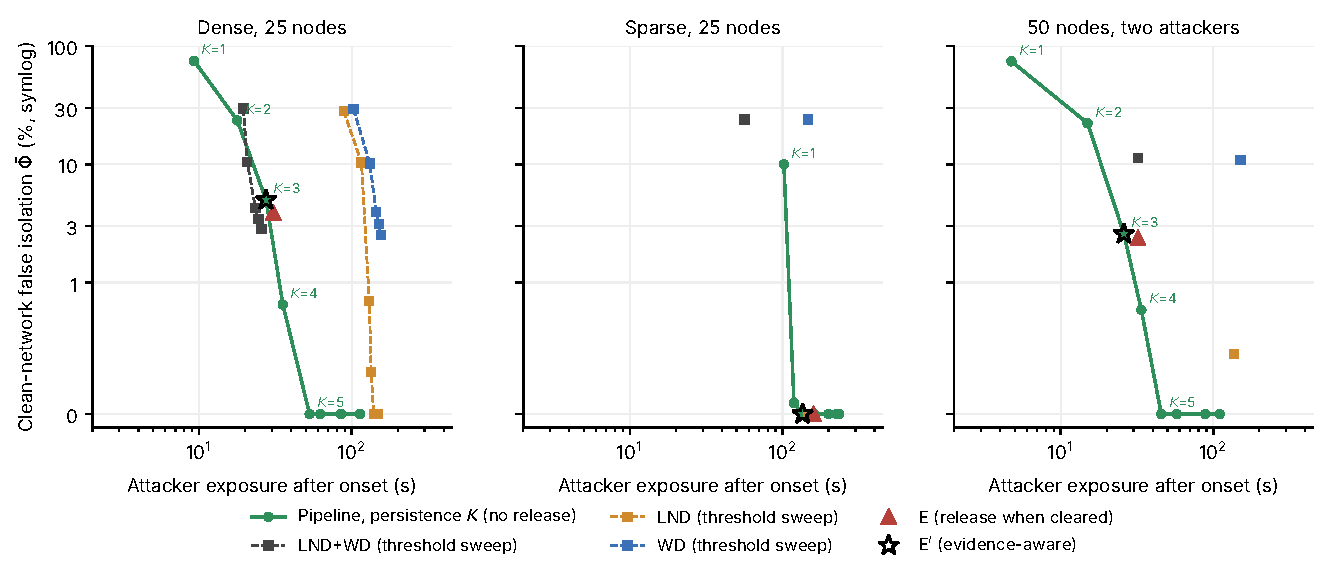
\includegraphics[width=\textwidth]{fig11_frontier}
\caption{Clean-network false isolation against attacker exposure for every
policy. Points towards the lower left are better on both axes. The green line
is the pipeline with persistence $K$ from 1 to 10 and no release; the star is
E$'$ and coincides with $K = 3$. Baselines are threshold sweeps in the dense
network and calibrated operating points elsewhere. Policies D and D$_w$ lie
above $K = 1$ and are omitted.}
\label{fig:frontier}
\end{figure}

\begin{table}[!t]
\caption{Selected points of Fig.~\ref{fig:frontier}. $\bar\Phi$ is clean-network
false isolation; exposure is the mean post-onset time an attacker is not
isolated, in seconds, over all attacked runs and for the forwarding-only
attacker A2. A point is Pareto-optimal (P) if no other policy in the same
network is at least as good on both axes and better on one.}
\label{tab:frontier}
\centering
\footnotesize
\setlength{\tabcolsep}{4pt}
\begin{tabular}{@{}llrrrc@{}}
\toprule
Network & Policy & $\bar\Phi$ (\%) & Exposure & Exposure A2 & P \\
\midrule
Dense & K$_1$ (= D$_1$) & 74.8 & 9.3 & 15.2 & \checkmark \\
      & K$_2$ & 23.5 & 17.8 & 26.3 & \checkmark \\
      & LND+WD, calibrated & 3.4 & 24.4 & 37.7 & \checkmark \\
      & E$'$ (= K$_3$) & 5.0 & 27.4 & 41.7 & \\
      & E & 3.9 & 30.6 & 51.2 & \\
      & K$_4$ & 0.8 & 35.3 & 55.3 & \checkmark \\
      & K$_5$ & 0.0 & 52.9 & 95.2 & \checkmark \\
      & LND, calibrated & 0.3 & 133.9 & 364.0 & \\
      & WD, calibrated & 3.1 & 150.3 & 37.7 & \\
Sparse & LND+WD & 23.9 & 56.2 & 100.0 & \checkmark \\
       & K$_1$ (= D$_1$) & 10.0 & 102.0 & 227.0 & \checkmark \\
       & E$'$ (= K$_3$) & 0.0 & 135.3 & 284.0 & \checkmark \\
       & E & 0.0 & 159.7 & 333.5 & \\
50-node & K$_2$ & 22.2 & 15.0 & 23.5 & \checkmark \\
        & E$'$ (= K$_3$) & 2.6 & 25.9 & 42.0 & \checkmark \\
        & E & 2.4 & 32.1 & 60.5 & \checkmark \\
        & LND+WD & 11.3 & 32.0 & 36.8 & \\
        & K$_4$ & 0.8 & 33.8 & 54.5 & \checkmark \\
\bottomrule
\end{tabular}
\end{table}

Three results follow. First, persistence alone moves the pipeline along the
whole frontier. In the dense network, raising $K$ from 1 to
5 lowered clean-network false isolation from 74.8\% to zero while mean
exposure rose from 9 to 53\,s, and the same shape appears in the 50-node
network. The immediate and confirmation-gated policies of
Section~\ref{sec:phi} are therefore not two designs but two settings of one
parameter, and the steep part of the curve lies between $K = 1$ and $K = 3$:
the second and third malicious windows remove most of the false isolation
for about 18\,s of extra exposure.

Second, which detector is on the frontier depends on the network, as
Sections~\ref{sec:baselines}--\ref{sec:scale} found separately. In the dense
network the calibrated LND+WD disjunction dominates E$'$ narrowly on point
estimates (3.4\% against 5.0\% false isolation, 24.4 against 27.4\,s
exposure; the paired false-isolation difference of Section~\ref{sec:baselines}
includes zero), and the
pipeline contributes the low-false-isolation end of the frontier ($K \ge 4$).
At 50 nodes E$'$ dominates LND+WD on both axes. In the sparse network the two
occupy opposite ends: LND+WD exposes attackers for less time but withdraws
nearly a quarter of honest-beacon service, while E$'$ withdraws none. The
single-evidence baselines are dominated everywhere, because the attack they
cannot see leaves its attacker exposed for the whole run.

Third, release adds exposure for little benefit. At the same isolation rule,
E exposed the forwarding attacker A2 for longer than E$'$ in every network
(51.2 against 41.7\,s dense, 333.5 against 284.0\,s sparse, 60.5 against
42.0\,s at 50 nodes) and lowered clean false isolation by at most 1.1
percentage points. These E figures come from the offline replay; in the closed
loop of Section~\ref{sec:release} E re-admits the A2 attacker in every seed,
so its true exposure is larger. A deployment should therefore choose the
persistence $K$ to suit the prior probability of attack and the cost of a lost
beacon, and should not rely on release to correct an aggressive setting.

\section{Discussion}
\label{sec:discussion}

\subsection{Interpretation}

The coverage result is structural, following from what each evidence class can
physically observe, and it was obtained
with calibration held fixed across all scenarios. The implication for the
literature is narrow but practical. An accuracy reported against
localisation-visible attacks is an accuracy over that subset of the attack
space. EMBN-MANET's threat model is confined to false-location behaviour by
design, so its figure is correct within its scope and we do not dispute it.
What we would ask of any such report is one additional line: which attack
classes the evidence can observe at all.

The isolation result is the paper's strongest: confirmation-gated isolation
withdrew 3.9--5.0\% of honest-beacon service against 74.8\% for the strongest
immediate policy, and the ordering held under attack, under shadowing and when
enforced. Its cost is the time an attacker remains active before
confirmation, a median of 15--27.5\,s, or 125--150\,s for selective forwarding
under shadowing. Whether that trade is favourable depends on the prior
probability of attack and the cost of a lost beacon: gating suits rare attacks
and sparse beacon coverage, because $\Phi$ accumulates continuously while
exposure is bounded by the confirmation delay, and immediate isolation suits
frequent attacks and high redundancy (Table~\ref{tab:guide}). The bound on
exposure holds only if release cannot be triggered by missing evidence, and in
our data the safe release rule made isolation on confirmation close to
permanent. We suggest that $\Phi$ or a comparable measure be reported
routinely, since a false-positive rate says nothing about how long errors
persist.

\begin{table}[!t]
\caption{Isolation policy by operating condition, as suggested by the results.}
\label{tab:guide}
\centering
\footnotesize
\begin{tabular}{@{}>{\raggedright\arraybackslash}p{4.4cm}>{\raggedright\arraybackslash}p{2.2cm}>{\raggedright\arraybackslash}p{5.4cm}@{}}
\toprule
Condition & Policy & Basis in the results \\
\midrule
Attacks rare, few redundant beacons & E$'$ & About 4--5\% of honest-beacon service withdrawn; attacker active for the confirmation delay \\
Attacks frequent, many redundant beacons & K$_1$ (D$_1$) or K$_2$ & Removes attackers soonest; K$_2$ withdraws 22--24\% of honest-beacon service against 60--75\% for D$_1$ \\
False isolation must be near zero & K$_4$ or K$_5$ & 0--0.8\% of honest-beacon service withdrawn, for 34--53\,s of attacker exposure \\
Forwarding-only attackers expected & E$'$, not E & E re-admits forwarding attackers once isolation silences their evidence \\
Sparse network & E$'$ with peer-relative behavioural scoring & No false isolation observed, but forwarding attackers confirmed in 4 of 10 seeds \\
Heavy shadowing & E$'$ & False isolation stays low; expect 2--3\,min to confirm forwarding attacks \\
\bottomrule
\end{tabular}
\end{table}

Two practical limits apply to this guidance. First, $\Phi$ counts lost
beacon service time, not metres of localisation error. Our runs did not
recompute the position estimates of nodes near a wrongly isolated beacon, so
the paper cannot convert one into the other; doing so needs the node density
around each beacon and the localisation algorithm in use. Second, the
pipeline falsely confirmed about one honest beacon in ten in the dense
network, and under E$'$ such isolations were almost never reversed. A
long-running deployment would lose beacons slowly, so it needs a planned
path back, such as the probationary release of Section~\ref{sec:future}.

The release finding is not specific to our pipeline. Any scheme that
restores trust as bad evidence fades has the same exposure, because an
isolated node produces no evidence at all. CONFIDANT's re-integration of
nodes whose reputation recovers over time~\cite{buchegger2002confidant} and
OCEAN's faulty-list timeout~\cite{bansal2003ocean} are examples: a forwarding
attacker excluded from routes stops generating the observations that would
keep its reputation low. Earlier critiques of redemption assumed that the
attacker waits out a timer or behaves well to rebuild its
score~\cite{sen2010survey,sun2006attacks}; here re-admission needs no action
by the attacker at all, which is why a defence against on--off behaviour
does not by itself prevent it.

\subsection{Limits of the evidence}

Whether fusion helped was decided by the attack family, not by the
combination rule. The same detector diluted a disjunctive rule when the
branches' sensitivity ratio was 3.63 and matched or slightly exceeded it at
1.87, as the $1+\sqrt2$ bound predicts. The baseline comparison is the same
result at the level of whole detectors: in the small dense network two
calibrated single-evidence detectors run in parallel matched the pipeline,
while in the sparse and 50-node networks they withdrew 11--24\% of
honest-beacon service against 0--3\%, through peer-relative scoring in the
first case and fusion in the second. When fusion helps, it does so by
suppressing single-branch false alarms, at the price of sensitivity near the
threshold. Branch sensitivity to an attack family can be measured before
fusion is applied, and no system we surveyed reports checking it; because an
adaptive adversary could concentrate its misbehaviour on one axis, a
single-branch path to confirmation should stay alongside the fused statistic.

The aggregation stage changed no verdict in the ablation (Online Resource~1,
Sect.~S6), so a system using only direct per-observer trust would reproduce
every reported finding. It remains as an unevaluated extension for conditions
our campaign barely samples: observers who disagree, noisy direct trust and
recommenders who lie. Neither isolation policy produced a defensible
throughput benefit, possibly because AODV finds alternative routes readily in
a dense 25-node topology~\cite{sirajuddin2021tbsmr,kavitha2019india,buksh2024trust};
on our evidence the claim that isolation restores network performance is
unsupported. Throughput says nothing about A1, which has no packet-level
footprint; localisation error is the appropriate metric for that attack.

\section{Threats to Validity}
\label{sec:threats}

\textbf{Construct validity.} The pipeline runs over logged simulator traces:
recommendation messages were not simulated (Section~\ref{sec:cost}), only the
resulting isolation schedules were enforced, and behavioural monitoring is
node-global rather than per-observer, which may explain the null aggregation
ablation. $\Phi$ for the 30-seed campaign assumes that an isolation does not
change later verdicts. This is exact for the first isolation of a
never-releasing policy but not for E's release times
(Section~\ref{sec:release}). Enforced replay on ten clean seeds moved neither
policy's $\Phi$ distinguishably from zero, and three closed-loop rounds left
E$'$ at a fixed point; iteration approximates an online detector but is not
one. E$'$ was designed after the enforced runs were examined, so only its
sparse and 50-node results (no attacker released, clean false isolation of 0
and 2.6\%) are out-of-sample. In the sparse calibration runs every usable
honest behavioural window forwarded all its transit packets, so the
behavioural scale collapsed to its floor; this makes the branch maximally
sensitive and cannot explain the low sparse detection rate, but the sparse
behavioural figures should be read with it in mind.

\textbf{Internal validity.} Thresholds were calibrated on held-out clean runs
and fixed, which avoids tuning to the test scenarios but gives no scenario its
optimal operating point. The recovery baseline window is short relative to
throughput variance, which is why throughput debt is excluded.

\textbf{External validity.} Detection and the false-isolation result survive
4--8\,dB shadowing, at a cost in latency for forwarding attacks, but the
channel has no multipath or obstruction model. Attackers do not collude or
adapt, mobility is synthetic, and only the hybrid attack's intensity is swept.
The throughput nulls rest on the small dense field alone. Memory limited the
network size: a 50-node run needs about 3\,GB, and a 100-node configuration
did not fit. Three monitored beacons per run, six at 50 nodes, make
rate-based metrics coarse. We do not claim generality beyond this
configuration.

\textbf{Comparative validity.} The baselines re-implement the evidence class
and decision rule of Liu--Ning--Du alert counting and watchdog/CONFIDANT
reputation on our counters and residual, with thresholds set by rules we
chose; a different defensible rule would move their operating points. Policies
D, D$_w$ and D$_1$ are our own constructions. In Section~\ref{sec:frontier}
the persistence settings share D$_1$'s replay assumption, and baseline
exposure in the sparse and 50-node networks is estimated from detection counts
and latencies. The comparison with EMBN-MANET is analytical.

\textbf{Statistical conclusion validity.} Coverage, latency, false positives
and $\Phi$ rest on 30 seeds with paired bootstrap intervals; throughput,
recovery, localisation error and the ablation on five; the sparse and 50-node
campaigns and the sweeps on ten, so the one-seed fusion gain is reported as
consistent with the condition, not as a benefit. About forty paired intervals
are reported without multiplicity correction. The central comparisons
(immediate policies against E or E$'$) lie hundreds of node-seconds from zero;
intervals that only just exclude or touch zero, such as several 50-node
baseline comparisons, are indicative.

\section{Conclusion}
\label{sec:conclusion}

Across 780 ns-3 runs, single-evidence detection of malicious beacons was blind
to attacks outside its evidence class, and collecting both behavioural and
localisation evidence removed the observed blind spots. Confirmation-gated
isolation withdrew 3.9\% of honest-beacon service on a clean network against
74.8\% for the strongest immediate policy, at a median cost of 15--27.5\,s of
attacker activity, and the confirmation persistence alone traced the
trade-off between the two. Releasing a beacon when its verdict clears
re-admitted forwarding attackers, whose behavioural evidence disappears while
they are isolated; requiring that evidence to return prevented every
re-admission and raised false isolation only to 5.0\%. These results held
under 4 and 8\,dB shadowing, with the price moving to latency. A condition on
the branches' relative sensitivity predicted when Stouffer fusion diluted or
matched a disjunctive rule, and explains why two calibrated literature
baselines run side by side matched the pipeline in a small dense network but
withdrew 11--24\% of honest-beacon service, against 0--3\%, in sparse and
larger ones. The aggregation stage changed no verdict, and no isolation policy
produced a measurable throughput gain. In a literature where reported
accuracies cluster between 90 and 99\%, the more informative questions are
which attacks a detector can see and how long its mistakes last.

\subsection{Future work}
\label{sec:future}

Three directions follow from these results. The first is to run the detector
inside the simulator, so that every isolation and release feeds back into
later verdicts. That would test the evidence-aware release rule without the
replay assumption, and it would allow a probationary release in which a
released beacon is isolated again on its first malicious window. The second
is to test the findings in harder settings: networks of 100 nodes or more,
trace-based mobility, colluding or adaptive attackers, and enforced
isolation in sparse topologies, where isolation is most likely to affect
delivery. Full implementations of EMBN-MANET and of a behavioural
trust-routing scheme belong in the same study. The third is to speed up
behavioural confirmation, which dominated latency under shadowing. A second
behavioural observable, or a confidence weight that adapts to the channel,
could shorten the time to confirm forwarding attacks.

\section*{Acknowledgements}

The authors thank the developers and maintainers of the ns-3 network
simulator~\cite{ns3}, whose simulator and AODV, IEEE 802.11 and propagation
models this study builds on, and the developers of the open-source Python
scientific stack used for the analysis.

\section*{Declarations}

\textbf{Funding.} No funding was received for this work.

\textbf{Competing interests.} The authors declare no competing interests.

\textbf{Author contributions.} A.V.\ designed and implemented the simulator,
verification pipeline and experiments, and drafted the manuscript. D.V.C.\
supervised the work, contributed to the experimental design and revised the
manuscript. Both authors read and approved the final version.

\textbf{Supplementary information.} Online Resource~1 contains the
intensity-sweep tables, supplementary figures and secondary analyses cited in
the text.

\textbf{Data and code availability.} Simulation sources, the analysis
pipeline, the scripts that run every campaign and regenerate every data
figure, and the result tables, per-window verdicts and isolation schedules
for every campaign are available at
\url{https://github.com/kraghu356/manet-beacon-trust}. The raw per-run
simulator traces are available from the corresponding author
on reasonable request. No third-party dataset was used: every data point in
this paper was generated by the authors' simulations.

\textbf{Use of AI tools.} An AI assistant (Claude, Anthropic) was used for
code analysis.

\textbf{Ethics approval.} Not applicable. This study involves neither human
participants nor animals.

\bibliography{sn-bibliography}

\end{document}
